\begin{frame}
\end{frame}

\begin{frame}{Motivation}
\protect\hypertarget{motivation}{}
Estimation and inference for a regression model depend on several
assumptions. The three main categories of assumptions are:

\textbf{Model}: The structural (mean) part of the model is correct,
i.e., \(E(y)=X\beta\).

\textbf{Error}: \(\epsilon\sim N(0,\sigma^2 I)\), i.e., that the errors
are normally distributed, independent, and identically distributed with
mean 0 and variance \(\sigma^2\).

\textbf{Unusual observations}: All observations should be equally
reliable and have approximately equal role in determining the regression
results and in influencing conclusions.
\end{frame}

\begin{frame}{Using Residuals to Check Error Assumptions}
\protect\hypertarget{using-residuals-to-check-error-assumptions}{}
Assumptions for \(\epsilon\) are tricky to check because \(\epsilon\) is
not observed.

Assumptions for \(\epsilon\) allow us to derive expected properties for
our residuals, \(\hat{\epsilon}\).

\begin{itemize}
\tightlist
\item
  The residuals are NOT interchangeable with the errors and have
  different properties.
\end{itemize}

Assumptions for ϵ are checked using \(\hat{\epsilon}\).

\begin{itemize}
\tightlist
\item
  If the observed residual behavior doesn't match the expected behavior,
  we believe this was caused by a violation of the relevant error
  assumption.
\end{itemize}
\end{frame}

\begin{frame}{Fact about OLS Residuals}
\protect\hypertarget{fact-about-ols-residuals}{}
\begin{itemize}
\tightlist
\item
  If \(E(\epsilon)=0\), then \(E(\hat{\epsilon}) = 0.\)
\item
  If \(var(\epsilon)=\sigma^2 I\), i.e., the errors are uncorrected and
  have constatn variance, then \(var(\hat{\epsilon}) = \sigma^2(I-H)\),
  where \(H = X(X^TX)^{-1}X^T\) is the hat matrix.
\item
  If \(E(\epsilon)=0\) and \(var(\epsilon)=\sigma^2I\), then
  \(cov(\hat{\epsilon}, \hat{y})=0_{n\times n}.\)
\item
  If \(x_i\) is the \(i\)th regressor, then
  \(cov(\hat{\epsilon}, x_i)=0\).
\item
  If an intercept is included in the fitted model, then
  \(\sum \hat{\epsilon}_i=0\).
\end{itemize}
\end{frame}

\begin{frame}{Checking the mean zero error assumption}
\protect\hypertarget{checking-the-mean-zero-error-assumption}{}
The mean zero assumption means that the average deviation of each error
from the true regression model is zero.

\begin{itemize}
\tightlist
\item
  Since we only observe a single value for each residual, we assess this
  assumption using the set of all residuals.
\end{itemize}

If the mean-zero error assumption is reasonable, then a plot of
\(\hat{\epsilon}\) versus \(\hat{y}\) or \(\hat{\epsilon}\) versus
\(x_i\) should be approximately symmetric around zero.

\begin{itemize}
\tightlist
\item
  This check implicitly assumes \(E(y)=X\beta\) and the errors are
  uncorrelated.
\end{itemize}

If the mean-zero error assumption is violated, then a plot of
\(\hat{\epsilon}\) versus \(\hat{y}\) or \(x_i\) will have a systematic,
asymmetrical pattern deviating from zero.
\end{frame}

\begin{frame}{Null Plot}
\protect\hypertarget{null-plot}{}
\begin{center}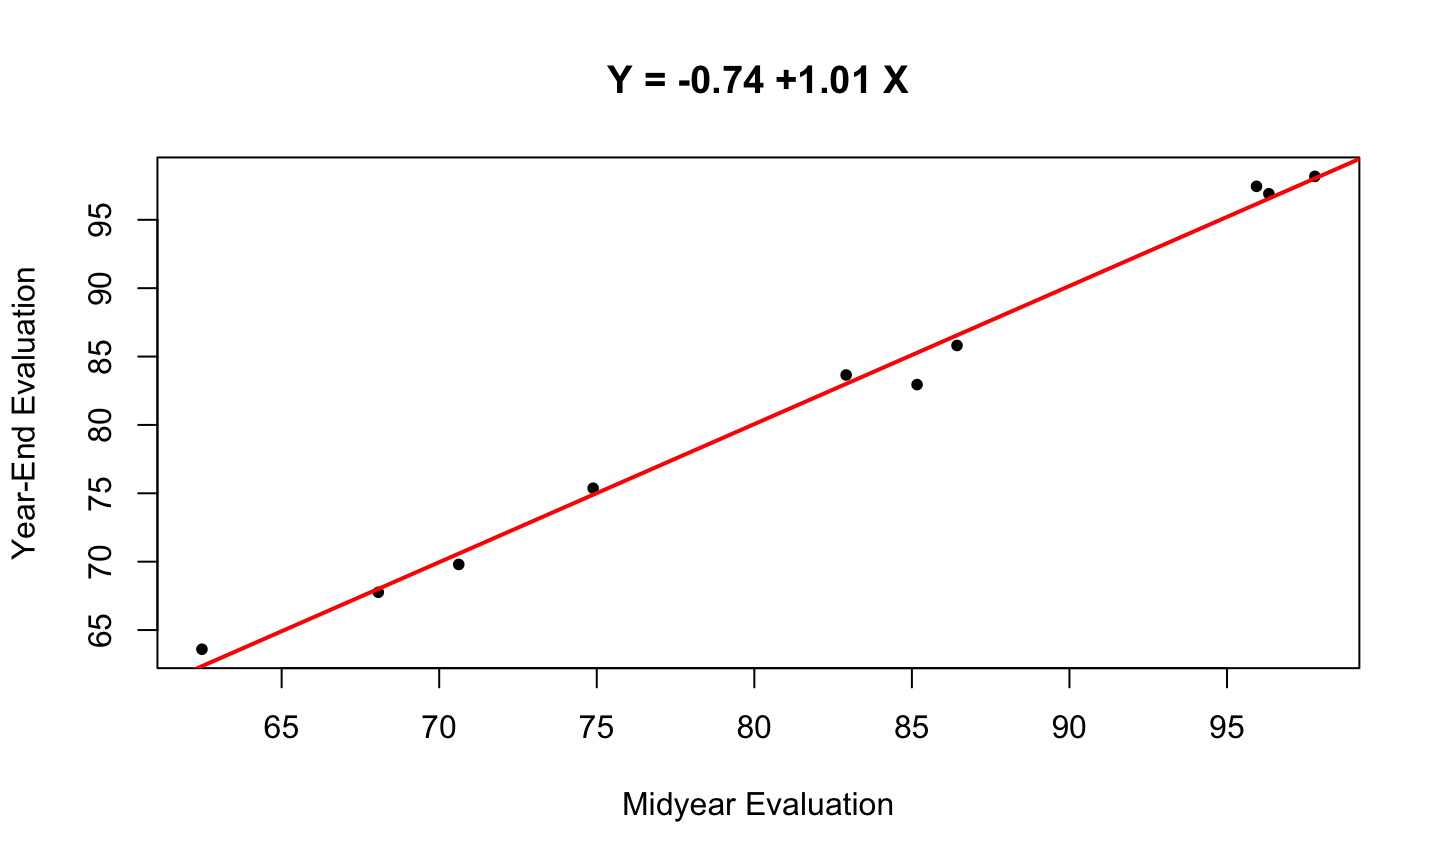
\includegraphics{error_assumption_files/figure-beamer/unnamed-chunk-1-1} \end{center}
\end{frame}

\begin{frame}[fragile]{Mean-zero assumption is violated}
\protect\hypertarget{mean-zero-assumption-is-violated}{}
\begin{Shaded}
\begin{Highlighting}[]
\NormalTok{x \textless{}{-}}\StringTok{ }\KeywordTok{seq}\NormalTok{(}\OperatorTok{{-}}\DecValTok{3}\NormalTok{,}\DecValTok{3}\NormalTok{,}\DataTypeTok{length.out =} \DecValTok{200}\NormalTok{)}
\NormalTok{y\textless{}{-}}\KeywordTok{c}\NormalTok{()}
\NormalTok{y[}\DecValTok{1}\OperatorTok{:}\DecValTok{50}\NormalTok{] \textless{}{-}}\StringTok{ }\DecValTok{2}\OperatorTok{*}\NormalTok{x[}\DecValTok{1}\OperatorTok{:}\DecValTok{50}\NormalTok{] }\OperatorTok{+}\StringTok{ }\KeywordTok{rnorm}\NormalTok{(}\DecValTok{50}\NormalTok{)}
\NormalTok{y[}\DecValTok{51}\OperatorTok{:}\DecValTok{100}\NormalTok{] \textless{}{-}}\StringTok{ }\DecValTok{2}\OperatorTok{*}\NormalTok{x[}\DecValTok{51}\OperatorTok{:}\DecValTok{100}\NormalTok{] }\OperatorTok{+}\StringTok{ }\KeywordTok{rnorm}\NormalTok{(}\DecValTok{50}\NormalTok{, }\DataTypeTok{mean =} \DecValTok{{-}4}\NormalTok{)}
\NormalTok{y[}\DecValTok{101}\OperatorTok{:}\DecValTok{150}\NormalTok{] \textless{}{-}}\StringTok{ }\DecValTok{2}\OperatorTok{*}\NormalTok{x[}\DecValTok{101}\OperatorTok{:}\DecValTok{150}\NormalTok{] }\OperatorTok{+}\StringTok{ }\KeywordTok{rnorm}\NormalTok{(}\DecValTok{50}\NormalTok{, }\DataTypeTok{mean =} \DecValTok{8}\NormalTok{)}
\NormalTok{y[}\DecValTok{151}\OperatorTok{:}\DecValTok{200}\NormalTok{] \textless{}{-}}\StringTok{ }\DecValTok{2}\OperatorTok{*}\NormalTok{x[}\DecValTok{151}\OperatorTok{:}\DecValTok{200}\NormalTok{] }\OperatorTok{+}\StringTok{ }\KeywordTok{rnorm}\NormalTok{(}\DecValTok{50}\NormalTok{, }\DataTypeTok{mean =}\DecValTok{12}\NormalTok{)}
\NormalTok{lmod =}\StringTok{ }\KeywordTok{lm}\NormalTok{(y}\OperatorTok{\textasciitilde{}}\NormalTok{x)}
\KeywordTok{plot}\NormalTok{(lmod}\OperatorTok{$}\NormalTok{residuals }\OperatorTok{\textasciitilde{}}\StringTok{ }\NormalTok{lmod}\OperatorTok{$}\NormalTok{fitted.values, }\DataTypeTok{main =} \StringTok{\textquotesingle{}Residuals vs Fitted Values\textquotesingle{}}\NormalTok{, }\DataTypeTok{xlab =} \StringTok{\textquotesingle{}Fitted Values\textquotesingle{}}\NormalTok{, }\DataTypeTok{ylab =}\StringTok{\textquotesingle{}residuals\textquotesingle{}}\NormalTok{)}
\end{Highlighting}
\end{Shaded}

\begin{center}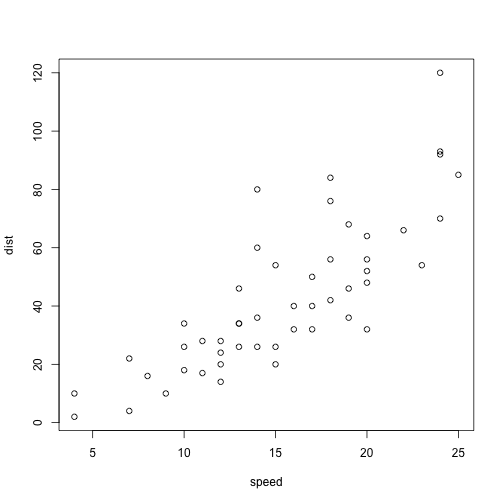
\includegraphics{error_assumption_files/figure-beamer/unnamed-chunk-2-1} \end{center}
\end{frame}

\begin{frame}[fragile]{Hold On}
\protect\hypertarget{hold-on}{}
\begin{Shaded}
\begin{Highlighting}[]
\NormalTok{x \textless{}{-}}\StringTok{ }\KeywordTok{seq}\NormalTok{(}\OperatorTok{{-}}\DecValTok{3}\NormalTok{,}\DecValTok{3}\NormalTok{,}\DataTypeTok{length.out =} \DecValTok{200}\NormalTok{)}
\NormalTok{y \textless{}{-}}\StringTok{ }\DecValTok{2}\OperatorTok{*}\NormalTok{x }\OperatorTok{+}\StringTok{ }\KeywordTok{rnorm}\NormalTok{(}\DecValTok{200}\NormalTok{, }\DataTypeTok{mean =} \DecValTok{500}\NormalTok{)}
\NormalTok{lmod =}\StringTok{ }\KeywordTok{lm}\NormalTok{(y}\OperatorTok{\textasciitilde{}}\NormalTok{x)}
\KeywordTok{plot}\NormalTok{(lmod}\OperatorTok{$}\NormalTok{residuals }\OperatorTok{\textasciitilde{}}\StringTok{ }\NormalTok{x, }\DataTypeTok{main =} \StringTok{\textquotesingle{}Where is the non{-}zero mean?\textquotesingle{}}\NormalTok{, }\DataTypeTok{xlab =} \StringTok{\textquotesingle{}Fitted Values\textquotesingle{}}\NormalTok{, }\DataTypeTok{ylab =}\StringTok{\textquotesingle{}residuals\textquotesingle{}}\NormalTok{)}
\KeywordTok{abline}\NormalTok{(}\DecValTok{0}\NormalTok{,}\DecValTok{0}\NormalTok{,}\DataTypeTok{col=}\StringTok{\textquotesingle{}red\textquotesingle{}}\NormalTok{)}
\end{Highlighting}
\end{Shaded}
\end{frame}

\begin{frame}{Hold On}
\protect\hypertarget{hold-on-1}{}
\begin{center}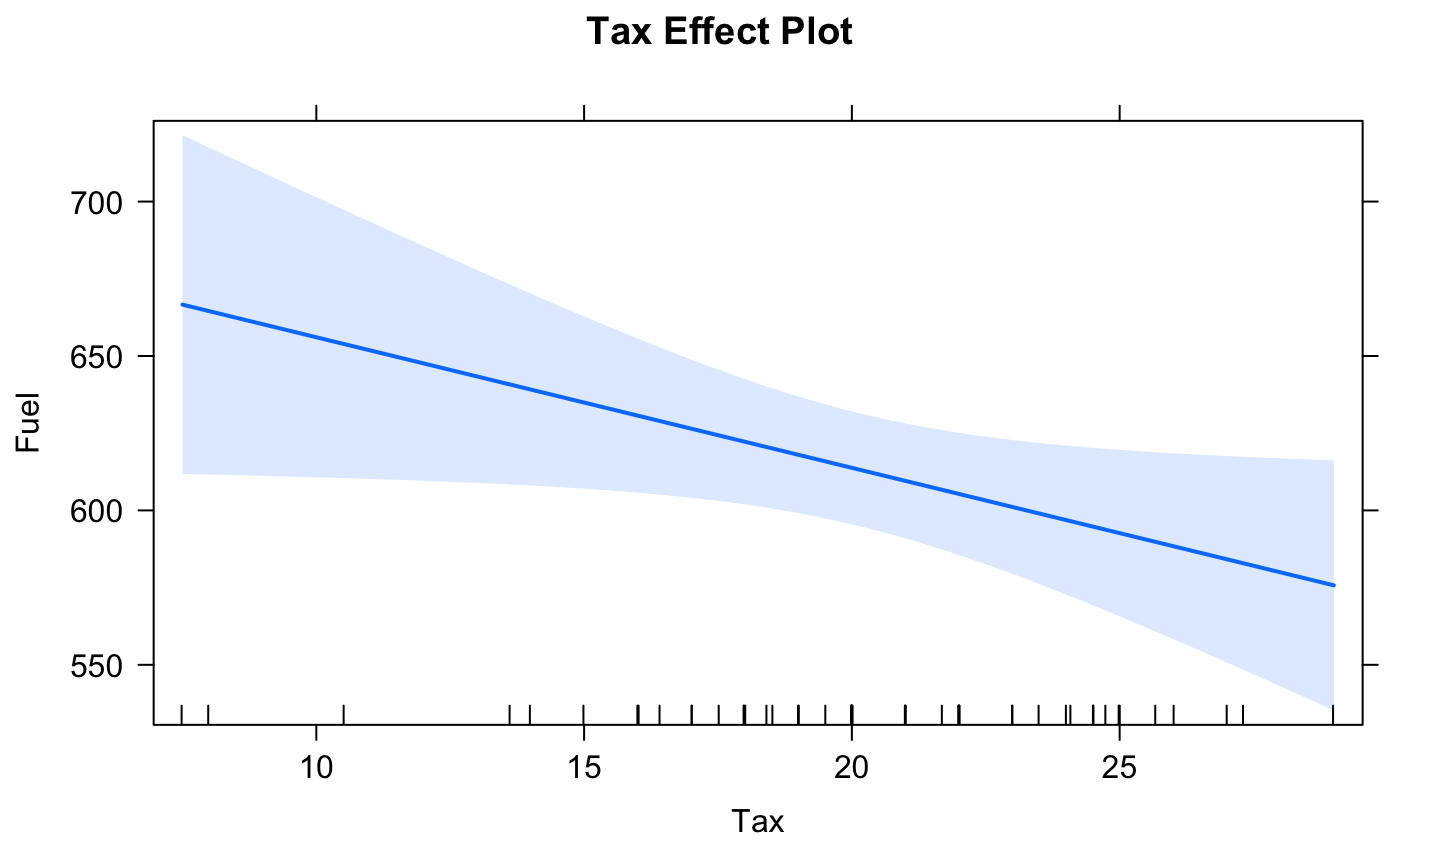
\includegraphics{error_assumption_files/figure-beamer/unnamed-chunk-4-1} \end{center}
\end{frame}

\begin{frame}{If Violation Detected}
\protect\hypertarget{if-violation-detected}{}
If a violation is detected, then you need to correct the structure of
your model.

\begin{itemize}
\tightlist
\item
  This may include transforming the response or predictors in the model.
\item
  This may include adding or deleting predictors from the model.
\item
  You may need to consider more advanced forms of regression.
\end{itemize}
\end{frame}

\begin{frame}[fragile]{Plotting in R}
\protect\hypertarget{plotting-in-r}{}
If the fitted R model is lmod:

\begin{itemize}
\tightlist
\item
  \texttt{car::residualPlot(lmod)} constructs a plot of
  \(\hat{\epsilon}\) versus \(\hat{y}\).
\item
  \texttt{car::residualPlots(lmod)} constructs plots of
  \(\hat{\epsilon}\) versus \(\hat{y}\) each each predictor.
\item
  \texttt{plot(lmod,\ which\ =\ 1)} construct a plot of
  \(\hat{\epsilon}\) versus \(\hat{y}\).
\end{itemize}
\end{frame}

\begin{frame}[fragile]{Savings Example}
\protect\hypertarget{savings-example}{}
The savings data frame in the faraway package includes 5 savings-related
variables in 50 countries averaged over the period 1960-1970:

\begin{itemize}
\tightlist
\item
  \texttt{sr} - savings rate. Personal saving divided by disposable
  income
\item
  \texttt{pop15} -- percentage of population under age of 15
\item
  \texttt{pop75} -- percentage of population over age of 75
\item
  \texttt{dpi} - per-capita disposable income in dollars
\item
  \texttt{ddpi} - percent growth rate of \texttt{dpi}
\end{itemize}

Is the mean-zero error assumption reasonable for the model regressing
\texttt{sr} on the other four variables?

\begin{Shaded}
\begin{Highlighting}[]
\KeywordTok{data}\NormalTok{(savings, }\DataTypeTok{package =} \StringTok{"faraway"}\NormalTok{)}
\NormalTok{lmod =}\StringTok{ }\KeywordTok{lm}\NormalTok{(sr }\OperatorTok{\textasciitilde{}}\StringTok{ }\NormalTok{., }\DataTypeTok{data =}\NormalTok{ savings)}
\KeywordTok{library}\NormalTok{(car)}
\end{Highlighting}
\end{Shaded}
\end{frame}

\begin{frame}[fragile]{Residuals vs.~Fitted Values}
\protect\hypertarget{residuals-vs.-fitted-values}{}
\begin{Shaded}
\begin{Highlighting}[]
\KeywordTok{residualPlot}\NormalTok{(lmod, }\DataTypeTok{quadratic =} \OtherTok{FALSE}\NormalTok{)}
\end{Highlighting}
\end{Shaded}

\begin{center}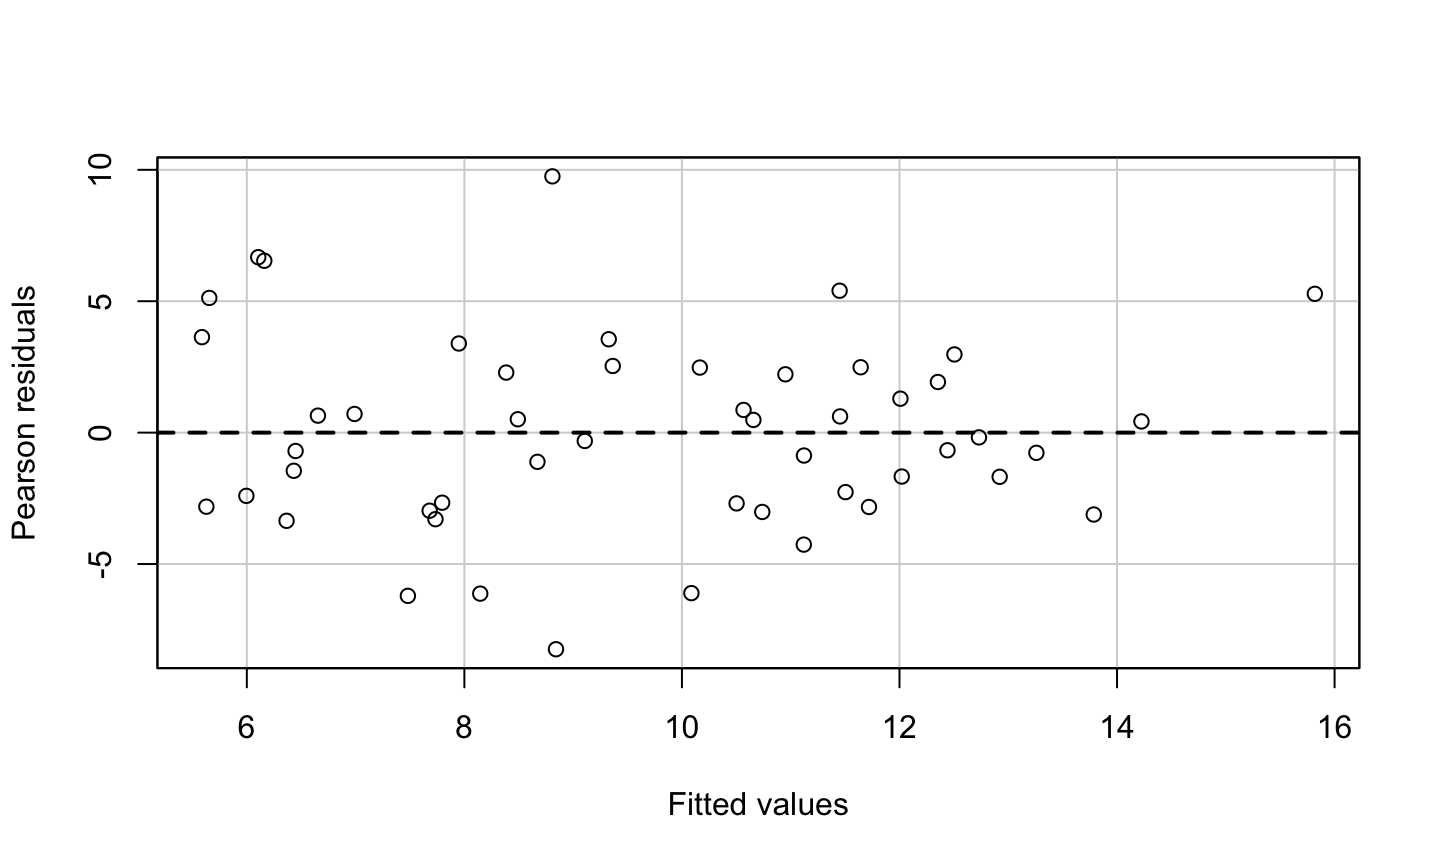
\includegraphics{error_assumption_files/figure-beamer/unnamed-chunk-6-1} \end{center}
\end{frame}

\begin{frame}[fragile]{plot of residuals versus fitted values}
\protect\hypertarget{plot-of-residuals-versus-fitted-values}{}
\begin{Shaded}
\begin{Highlighting}[]
\KeywordTok{plot}\NormalTok{(lmod, }\DataTypeTok{which =} \DecValTok{1}\NormalTok{)}
\end{Highlighting}
\end{Shaded}

\begin{center}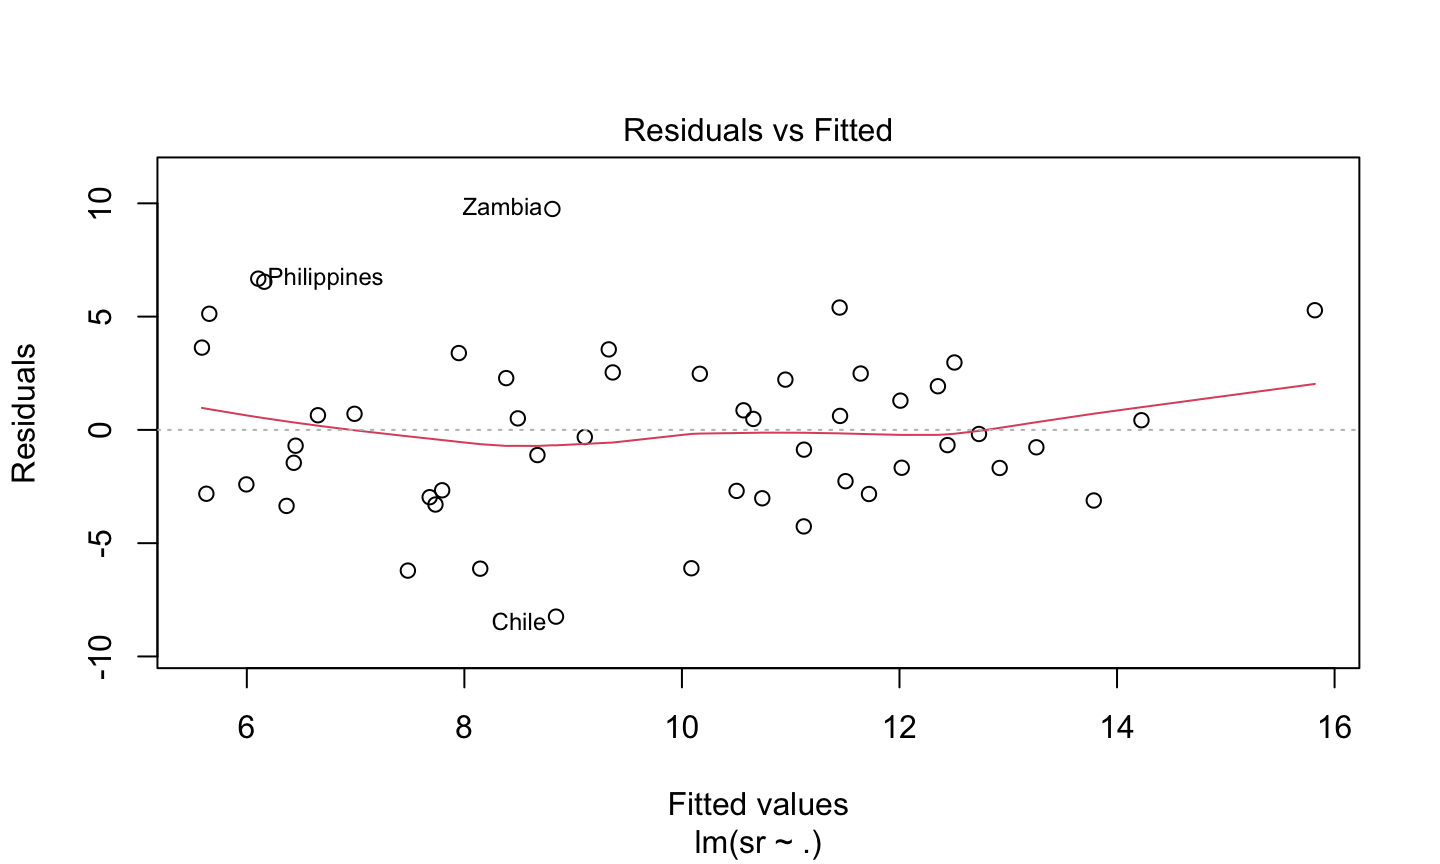
\includegraphics{error_assumption_files/figure-beamer/unnamed-chunk-7-1} \end{center}
\end{frame}

\begin{frame}[fragile]{plot of residuals versus predictors}
\protect\hypertarget{plot-of-residuals-versus-predictors}{}
\begin{Shaded}
\begin{Highlighting}[]
\KeywordTok{residualPlots}\NormalTok{(lmod, }\DataTypeTok{quadratic =} \OtherTok{FALSE}\NormalTok{, }\DataTypeTok{fitted =} \OtherTok{FALSE}\NormalTok{, }\DataTypeTok{tests =} \OtherTok{FALSE}\NormalTok{)}
\end{Highlighting}
\end{Shaded}

\begin{center}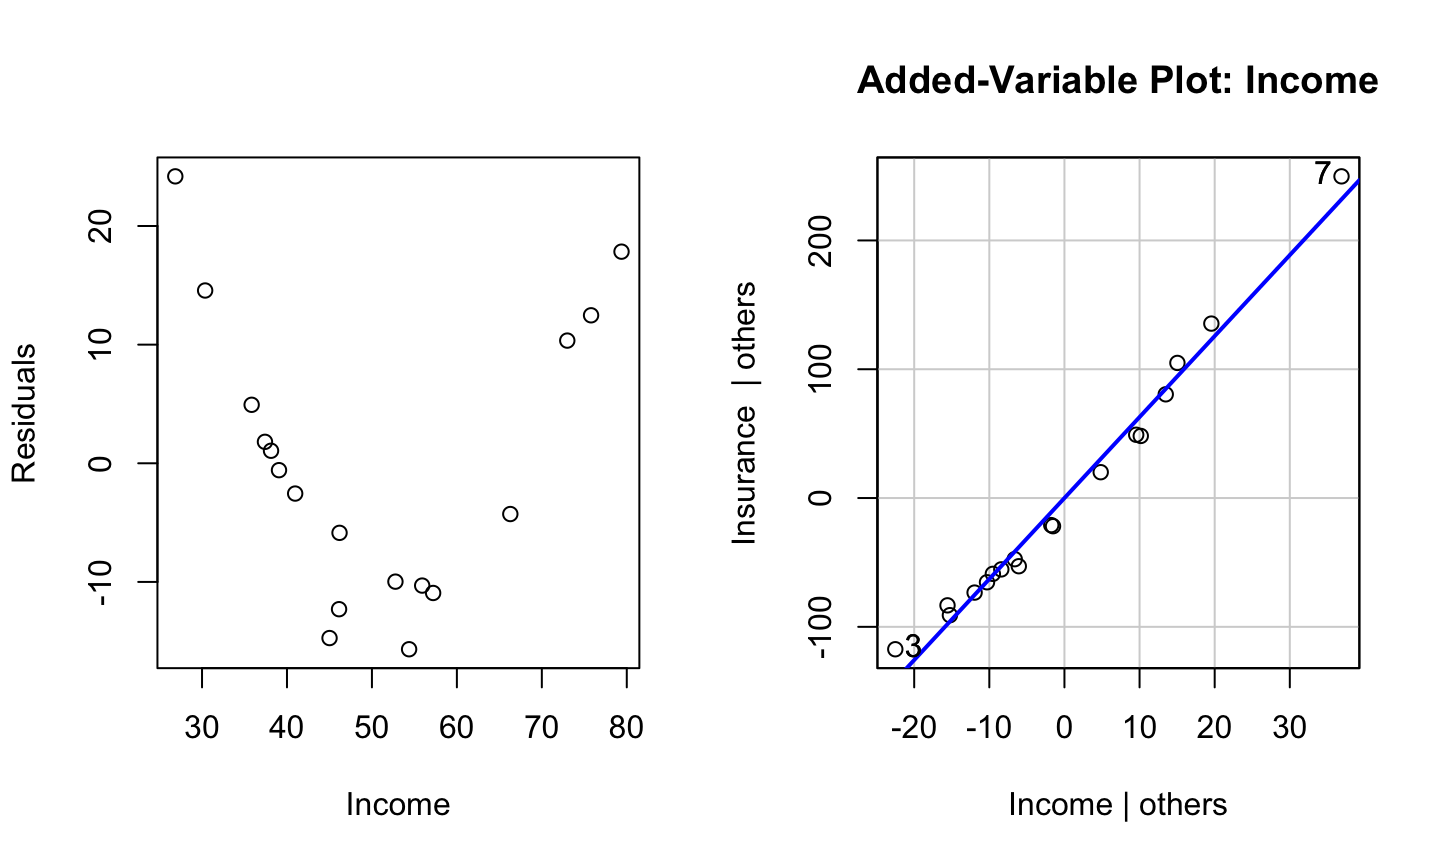
\includegraphics{error_assumption_files/figure-beamer/unnamed-chunk-8-1} \end{center}
\end{frame}

\begin{frame}{Symmetric, non-constant variance plot:}
\protect\hypertarget{symmetric-non-constant-variance-plot}{}
\begin{center}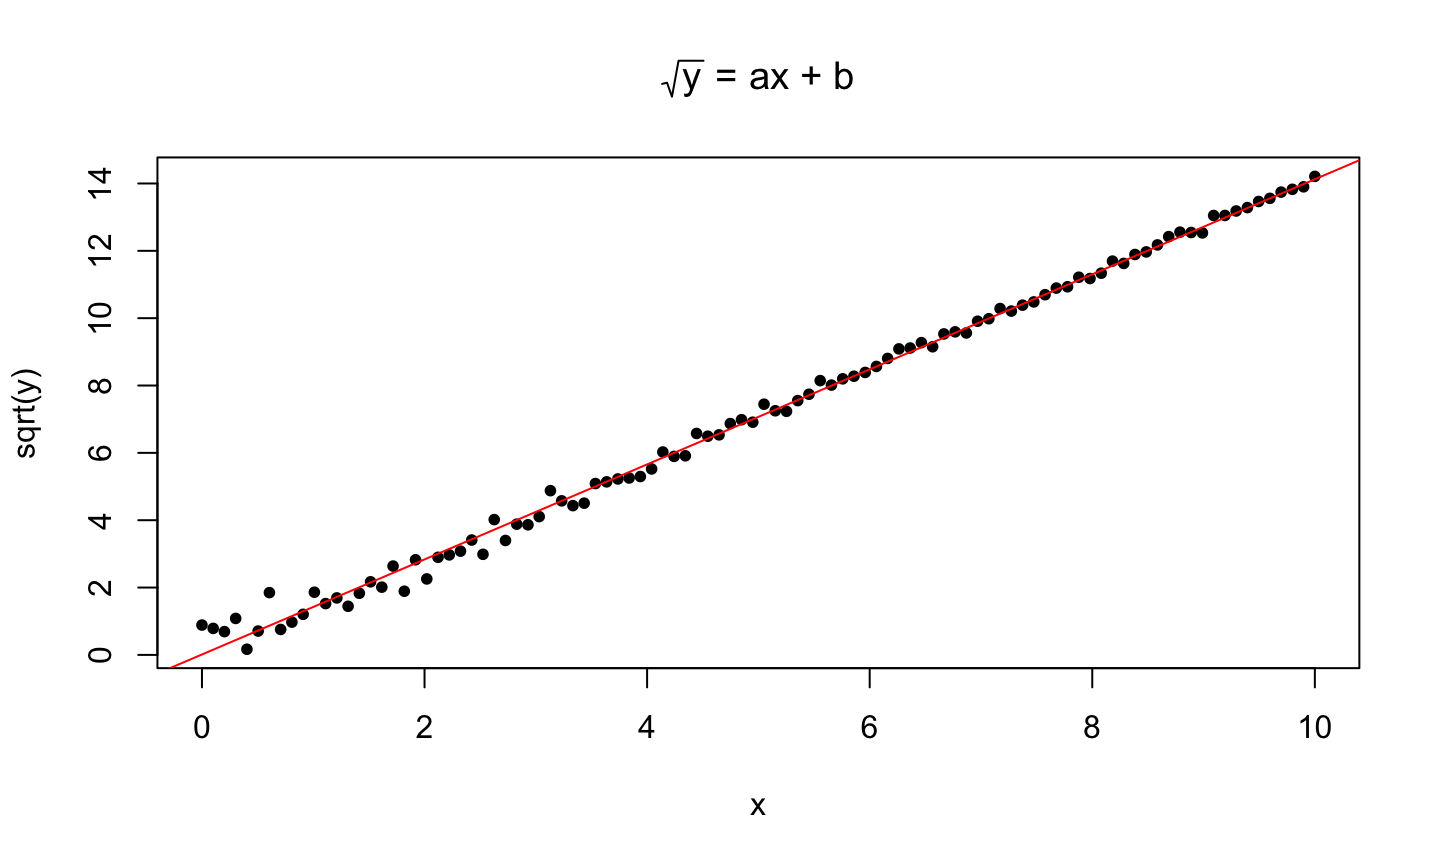
\includegraphics{error_assumption_files/figure-beamer/unnamed-chunk-9-1} \end{center}
\end{frame}

\begin{frame}[fragile]{Constant variance example}
\protect\hypertarget{constant-variance-example}{}
\begin{Shaded}
\begin{Highlighting}[]
\NormalTok{x\textless{}{-}}\KeywordTok{seq}\NormalTok{(}\DecValTok{1}\NormalTok{,}\DecValTok{100}\NormalTok{,}\DataTypeTok{length.out =} \DecValTok{200}\NormalTok{)}
\NormalTok{y \textless{}{-}}\StringTok{ }\DecValTok{5}\OperatorTok{*}\NormalTok{x }\DecValTok{{-}20} \OperatorTok{+}\StringTok{ }\KeywordTok{rnorm}\NormalTok{(}\DecValTok{200}\NormalTok{)}
\KeywordTok{plot}\NormalTok{(}\KeywordTok{lm}\NormalTok{(y}\OperatorTok{\textasciitilde{}}\NormalTok{x), }\DataTypeTok{which =} \DecValTok{3}\NormalTok{)}
\end{Highlighting}
\end{Shaded}

\begin{center}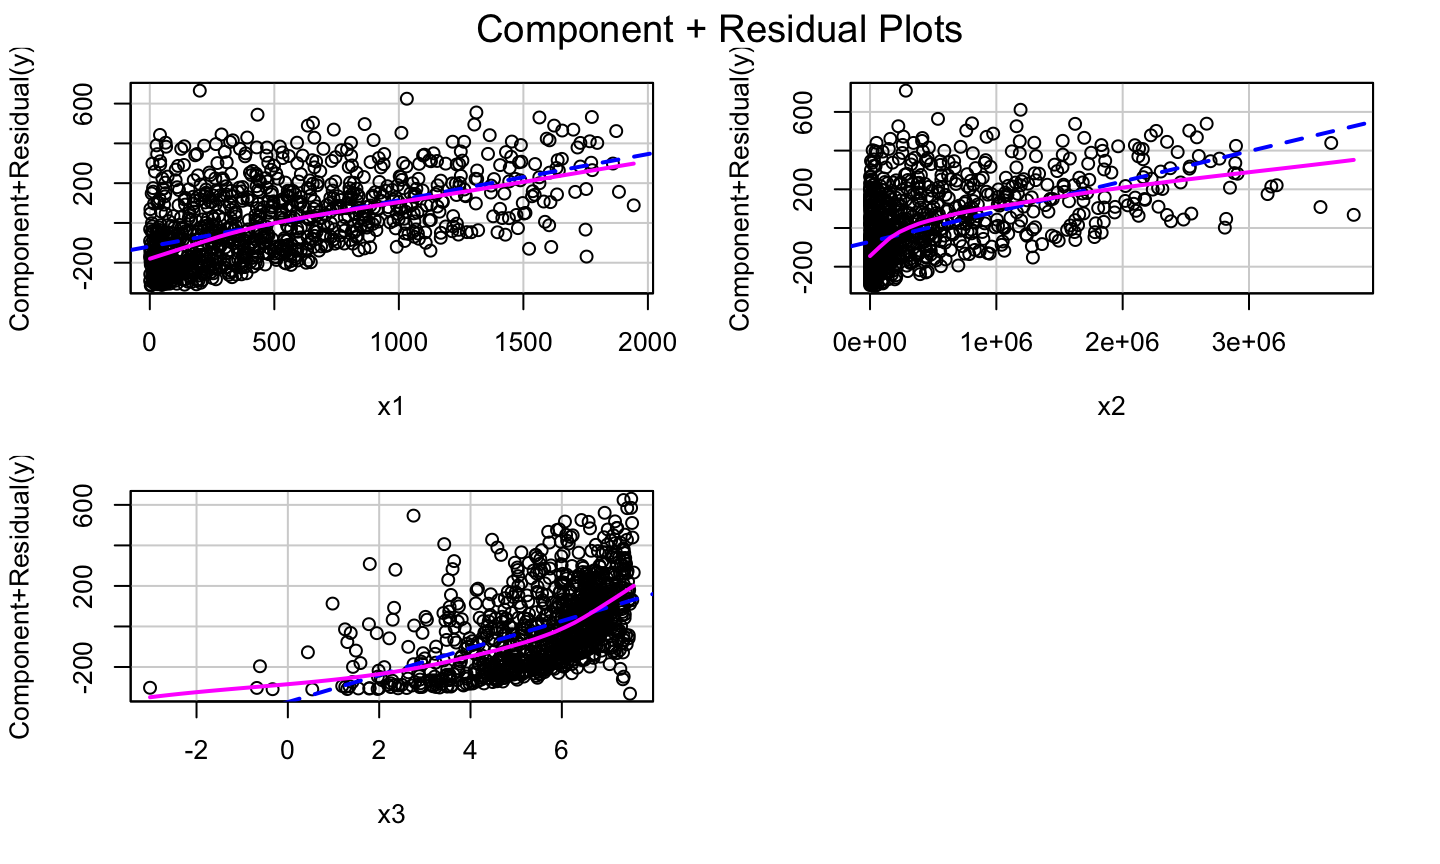
\includegraphics{error_assumption_files/figure-beamer/unnamed-chunk-10-1} \end{center}
\end{frame}

\begin{frame}[fragile]{Non-constat variance example}
\protect\hypertarget{non-constat-variance-example}{}
\begin{Shaded}
\begin{Highlighting}[]
\NormalTok{x\textless{}{-}}\KeywordTok{seq}\NormalTok{(}\DecValTok{1}\NormalTok{,}\DecValTok{100}\NormalTok{,}\DataTypeTok{length.out =} \DecValTok{200}\NormalTok{)}
\NormalTok{y \textless{}{-}}\StringTok{ }\DecValTok{5}\OperatorTok{*}\NormalTok{x }\DecValTok{{-}20}
\NormalTok{y =}\StringTok{ }\NormalTok{y }\OperatorTok{+}\StringTok{ }\KeywordTok{c}\NormalTok{(}\KeywordTok{rnorm}\NormalTok{(}\DecValTok{100}\NormalTok{,}\DecValTok{0}\NormalTok{, }\DecValTok{1}\NormalTok{), }\KeywordTok{rnorm}\NormalTok{(}\DecValTok{100}\NormalTok{, }\DecValTok{0}\NormalTok{, }\DecValTok{10}\NormalTok{))}
\NormalTok{lmod1 =}\StringTok{ }\KeywordTok{lm}\NormalTok{(y}\OperatorTok{\textasciitilde{}}\NormalTok{x)}
\KeywordTok{plot}\NormalTok{(lmod1, }\DataTypeTok{which =} \DecValTok{3}\NormalTok{)}
\end{Highlighting}
\end{Shaded}

\begin{center}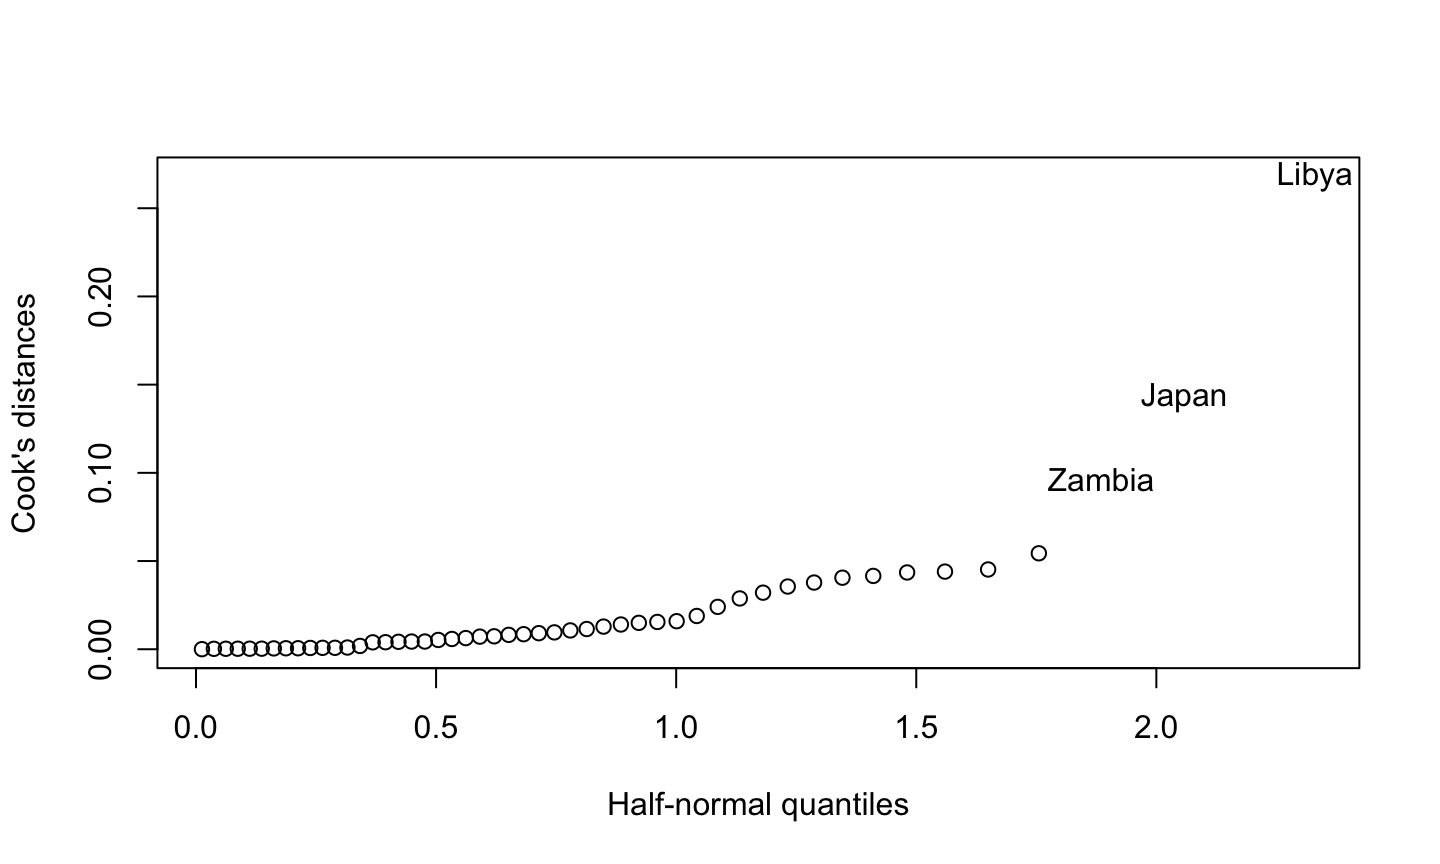
\includegraphics{error_assumption_files/figure-beamer/unnamed-chunk-11-1} \end{center}
\end{frame}

\begin{frame}[fragile]{Non-constant variance example}
\protect\hypertarget{non-constant-variance-example}{}
\begin{Shaded}
\begin{Highlighting}[]
\NormalTok{x1 \textless{}{-}}\StringTok{ }\KeywordTok{seq}\NormalTok{(}\DecValTok{1}\NormalTok{,}\DecValTok{100}\NormalTok{, }\DataTypeTok{length.out =} \DecValTok{200}\NormalTok{)}
\NormalTok{x2 \textless{}{-}}\StringTok{ }\KeywordTok{seq}\NormalTok{(}\DecValTok{1}\NormalTok{, }\DecValTok{10}\NormalTok{, }\DataTypeTok{length.out =} \DecValTok{200}\NormalTok{)}
\NormalTok{y \textless{}{-}}\StringTok{ }\DecValTok{5}\OperatorTok{*}\NormalTok{x1 }\OperatorTok{+}\StringTok{ }\DecValTok{2}\OperatorTok{*}\NormalTok{x2}\OperatorTok{\^{}}\DecValTok{2} \OperatorTok{{-}}\StringTok{ }\DecValTok{20} \OperatorTok{+}\StringTok{ }\KeywordTok{rnorm}\NormalTok{(}\DecValTok{200}\NormalTok{, }\DecValTok{0}\NormalTok{, }\DecValTok{5}\NormalTok{)}
\KeywordTok{plot}\NormalTok{(}\KeywordTok{lm}\NormalTok{(y}\OperatorTok{\textasciitilde{}}\NormalTok{x1), }\DataTypeTok{which =} \DecValTok{3}\NormalTok{)}
\end{Highlighting}
\end{Shaded}

\begin{center}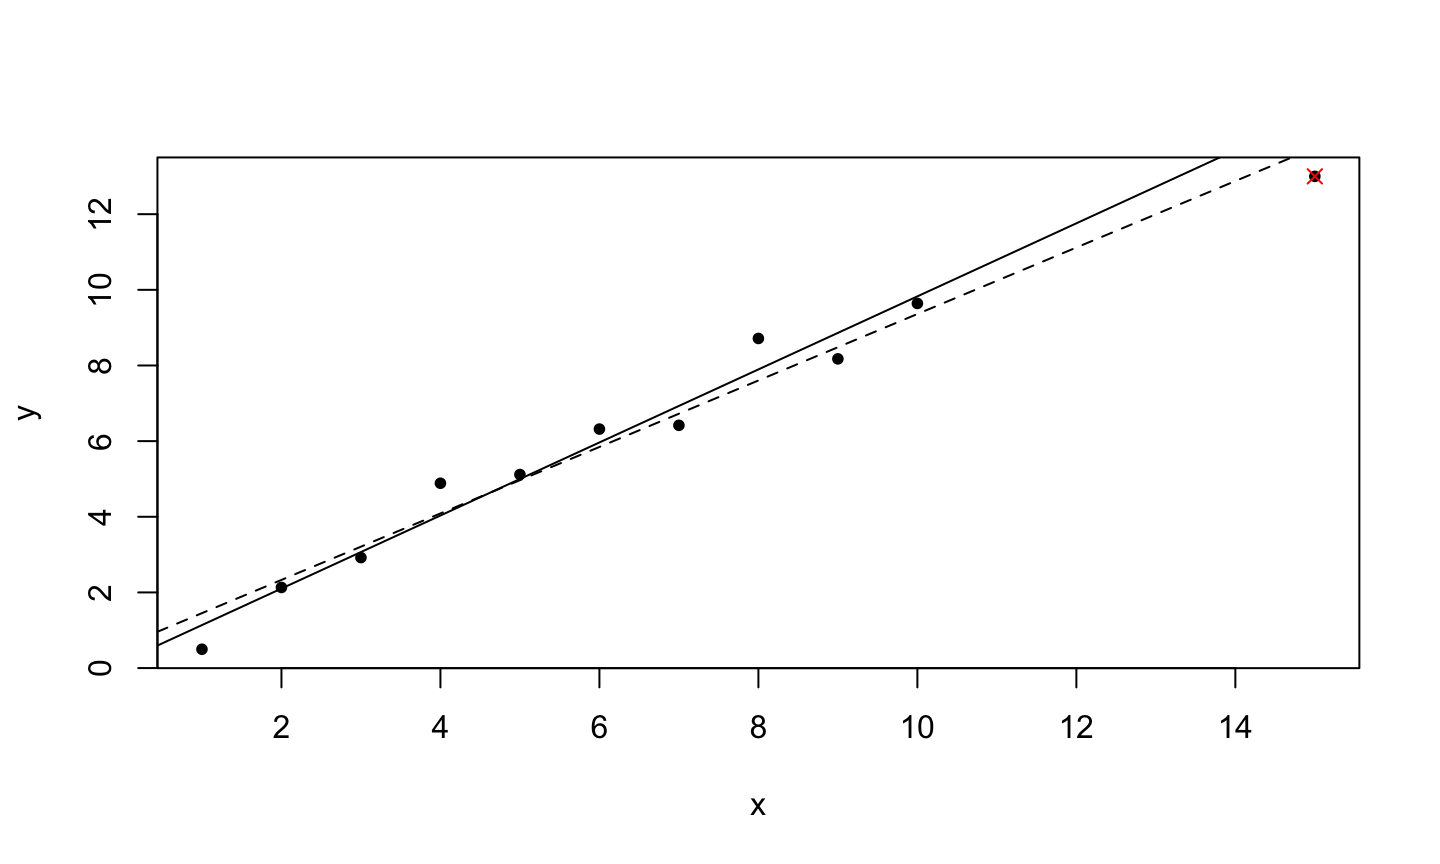
\includegraphics{error_assumption_files/figure-beamer/unnamed-chunk-12-1} \end{center}
\end{frame}

\begin{frame}{Checking for non-constant error variance}
\protect\hypertarget{checking-for-non-constant-error-variance}{}
The constant variance assumption means that the average squared
deviation of each error from the true regression model should be the
same for every observation.

\begin{itemize}
\tightlist
\item
  Since we only observe a single value for each residual, we assess this
  assumption using the set of all residuals.
\end{itemize}

If the constant error variance assumption is correct, then a plot of ϵ ̂
versus y ̂ or x\_i should be a random scatter of points and the spread
of the residuals should have a constant thickness as you move from left
to right along the x-axis of the plot.

\begin{itemize}
\tightlist
\item
  This check implicitly assumes the errors are uncorrelated.
\end{itemize}
\end{frame}

\begin{frame}{Non-constant variance}
\protect\hypertarget{non-constant-variance}{}
If the constant error variance assumption is violated, then a plot of
\(\hat{\epsilon}\) versus \(\hat{y}\) or \(x_i\) will have a systematic,
varying spread of the residuals.
\end{frame}

\begin{frame}[fragile]{plot sqrt absolute residuals vs fitted values}
\protect\hypertarget{plot-sqrt-absolute-residuals-vs-fitted-values}{}
\begin{Shaded}
\begin{Highlighting}[]
\KeywordTok{plot}\NormalTok{(lmod, }\DataTypeTok{which =} \DecValTok{3}\NormalTok{)}
\end{Highlighting}
\end{Shaded}

\begin{center}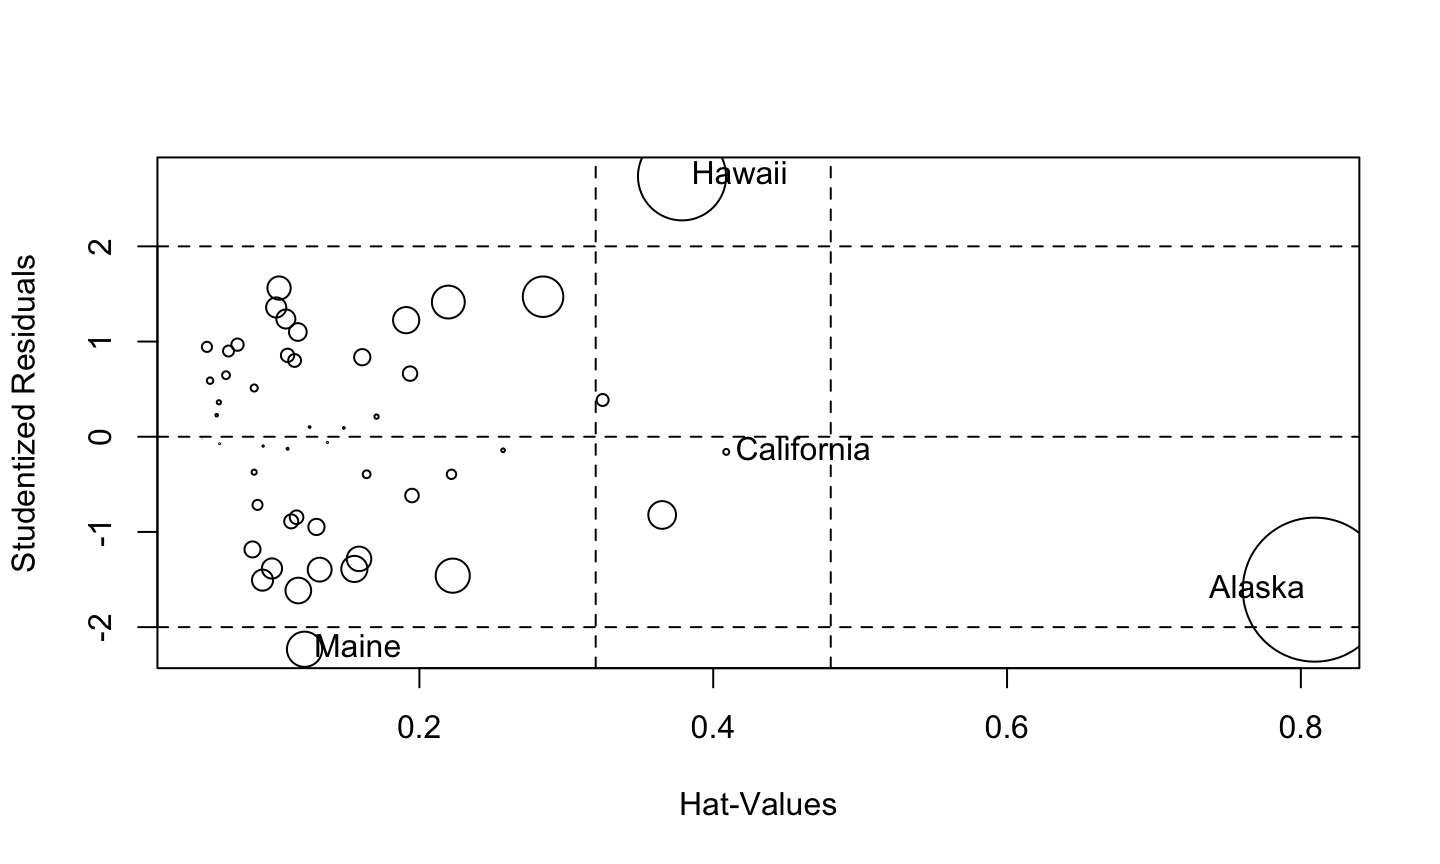
\includegraphics{error_assumption_files/figure-beamer/unnamed-chunk-13-1} \end{center}
\end{frame}

\begin{frame}{What we do?}
\protect\hypertarget{what-we-do}{}
If the non-constant error variance assumption is violated you should:

\begin{itemize}
\item
  Transformation of the response and/or predictors.
\item
  Square root and \(\log(y+c)\) transformations are common.
\item
  Transfomation of variables also correct for issues with model
  structure
\item
  Consider fitting a weighted least squares (WLS) regression model
  instead of OLS.
\item
  Specially when the structure is approximately correct
\item
  Example : when measurement error of the response depends on the
  response variable
\end{itemize}
\end{frame}

\begin{frame}{Galapagos Example}
\protect\hypertarget{galapagos-example}{}
\begin{center}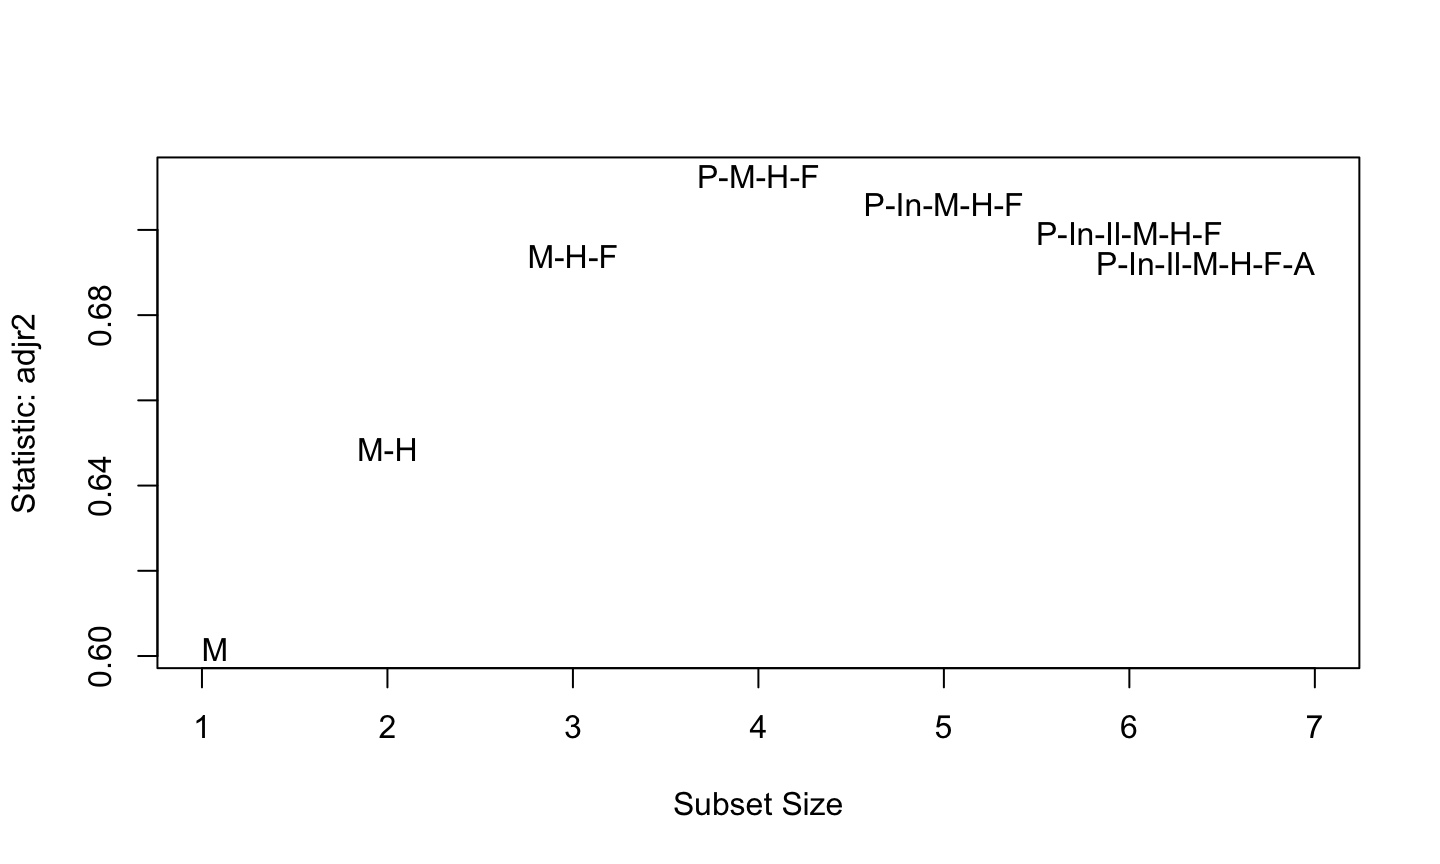
\includegraphics{error_assumption_files/figure-beamer/unnamed-chunk-14-1} \end{center}
\end{frame}

\begin{frame}[fragile]{Simulated Example}
\protect\hypertarget{simulated-example}{}
\begin{Shaded}
\begin{Highlighting}[]
\NormalTok{x1 =}\StringTok{ }\KeywordTok{seq}\NormalTok{(}\DecValTok{1}\NormalTok{,}\DecValTok{100}\NormalTok{,}\DataTypeTok{length.out =} \DecValTok{200}\NormalTok{)}
\NormalTok{y \textless{}{-}}\StringTok{ }\DecValTok{5}\OperatorTok{*}\NormalTok{x }\OperatorTok{{-}}\StringTok{ }\DecValTok{20} \OperatorTok{+}\StringTok{ }\KeywordTok{rnorm}\NormalTok{(}\DecValTok{200}\NormalTok{) }\CommentTok{\# Error for factor other than measurement }
\NormalTok{y \textless{}{-}}\StringTok{ }\NormalTok{y }\OperatorTok{+}\StringTok{ }\KeywordTok{rnorm}\NormalTok{(}\DecValTok{200}\NormalTok{, }\DecValTok{0}\NormalTok{, y}\OperatorTok{\^{}}\DecValTok{2}\OperatorTok{/}\DecValTok{10}\NormalTok{) }\CommentTok{\# Measurement error increase with y}
\KeywordTok{plot}\NormalTok{(x1,y)}
\end{Highlighting}
\end{Shaded}

\begin{center}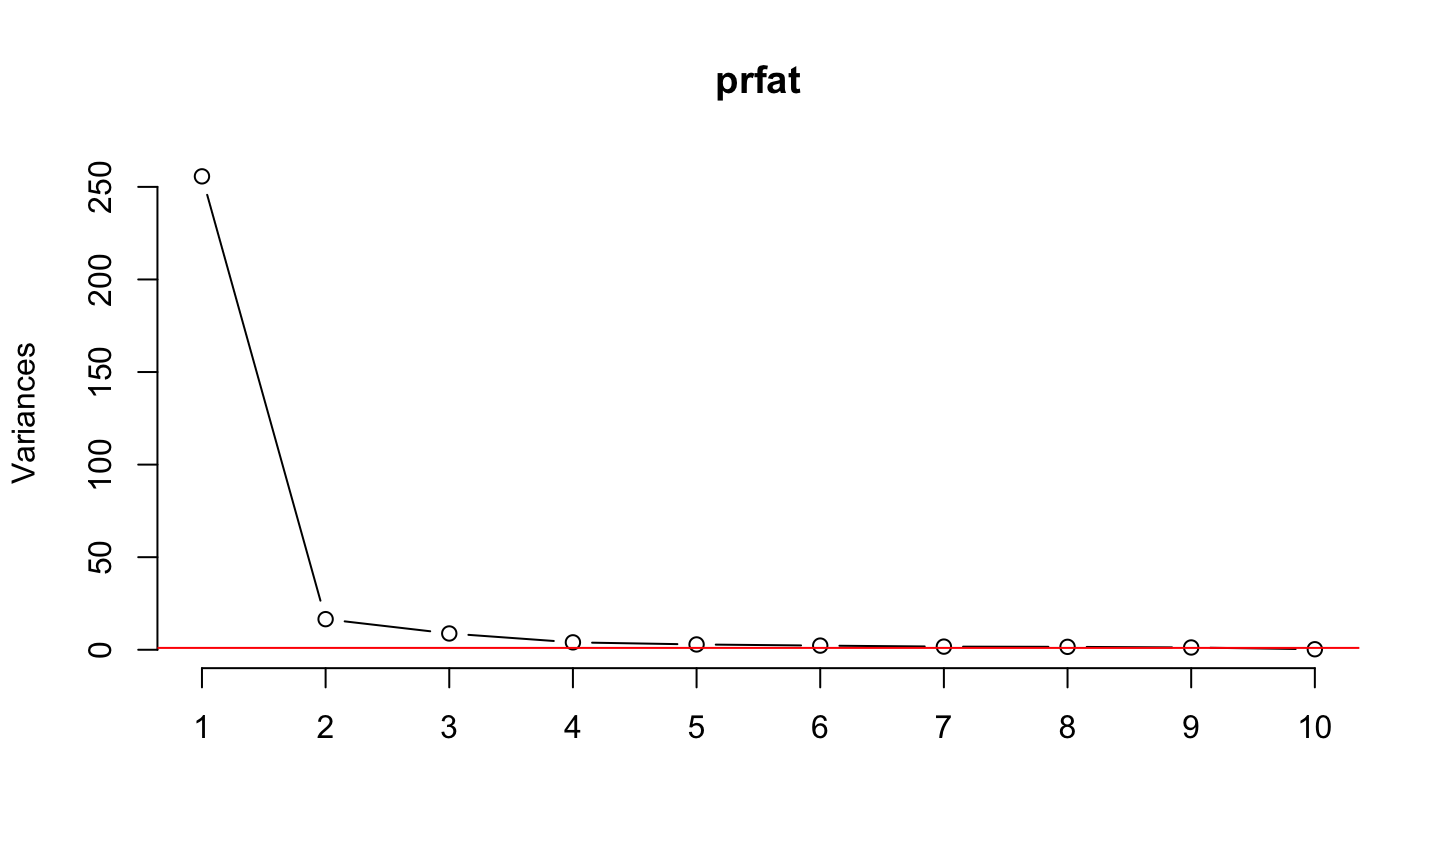
\includegraphics{error_assumption_files/figure-beamer/unnamed-chunk-15-1} \end{center}

Use WLS.
\end{frame}

\begin{frame}[fragile]{Savings Example}
\protect\hypertarget{savings-example-1}{}
\begin{Shaded}
\begin{Highlighting}[]
\KeywordTok{par}\NormalTok{(}\DataTypeTok{mfrow =} \KeywordTok{c}\NormalTok{(}\DecValTok{1}\NormalTok{,}\DecValTok{2}\NormalTok{))}
\KeywordTok{data}\NormalTok{(savings,}\DataTypeTok{package=}\StringTok{"faraway"}\NormalTok{)}
\NormalTok{lmod \textless{}{-}}\StringTok{ }\KeywordTok{lm}\NormalTok{(sr }\OperatorTok{\textasciitilde{}}\StringTok{ }\NormalTok{pop15}\OperatorTok{+}\NormalTok{pop75}\OperatorTok{+}\NormalTok{dpi}\OperatorTok{+}\NormalTok{ddpi,savings)}
\KeywordTok{plot}\NormalTok{(}\KeywordTok{fitted}\NormalTok{(lmod),}\KeywordTok{residuals}\NormalTok{(lmod),}\DataTypeTok{xlab=}\StringTok{"Fitted"}\NormalTok{,}\DataTypeTok{ylab=}\StringTok{"Residuals"}\NormalTok{)}
\KeywordTok{abline}\NormalTok{(}\DataTypeTok{h=}\DecValTok{0}\NormalTok{)}
\KeywordTok{plot}\NormalTok{(}\KeywordTok{fitted}\NormalTok{(lmod),}\KeywordTok{sqrt}\NormalTok{(}\KeywordTok{abs}\NormalTok{(}\KeywordTok{residuals}\NormalTok{(lmod))), }\DataTypeTok{xlab=}\StringTok{"Fitted"}\NormalTok{,}\DataTypeTok{ylab=}
    \KeywordTok{expression}\NormalTok{(}\KeywordTok{sqrt}\NormalTok{(}\KeywordTok{hat}\NormalTok{(epsilon))))}
\end{Highlighting}
\end{Shaded}

\begin{center}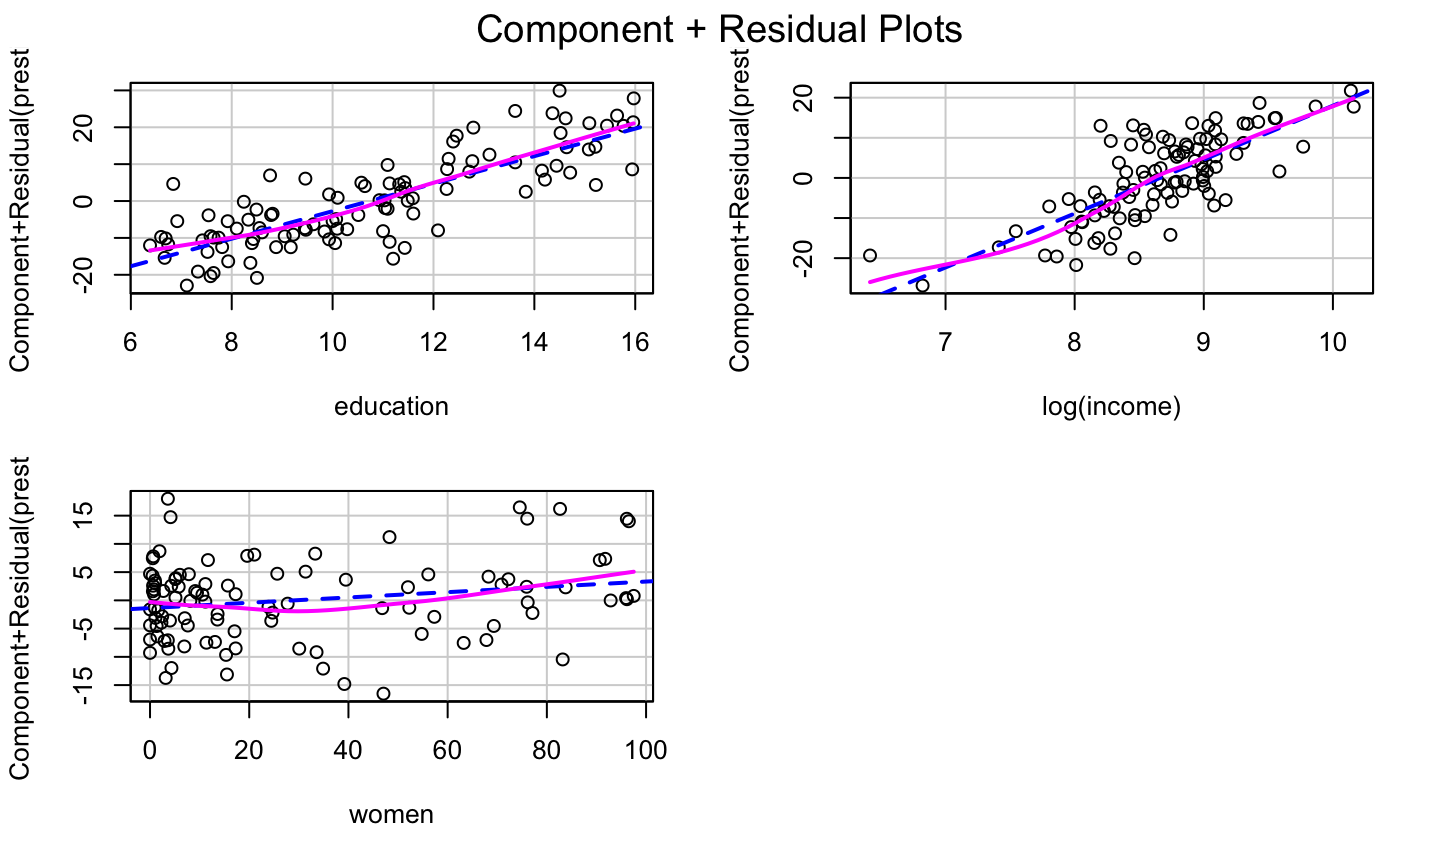
\includegraphics{error_assumption_files/figure-beamer/unnamed-chunk-16-1} \end{center}
\end{frame}

\begin{frame}{Test for equality of two variances}
\protect\hypertarget{test-for-equality-of-two-variances}{}
Suppose we have samples from two populations (\(Y = \{y_1,\dost y_n\}\)
and \(T = \{t_1, \dots t_m\}\)). We can test if the variances
\(\sigma_Y^2\) and \(\sigma_T^2\) are equal.

\begin{itemize}
\tightlist
\item
  Test statistic
\end{itemize}

\[\frac{S_Y^2}{S_T^2}\] * Distribution

The test statistic follows a \(F(n-1,m-1)\) distribution.
\end{frame}

\begin{frame}[fragile]{More into savings example}
\protect\hypertarget{more-into-savings-example}{}
\begin{Shaded}
\begin{Highlighting}[]
\KeywordTok{par}\NormalTok{(}\DataTypeTok{mfrow =} \KeywordTok{c}\NormalTok{(}\DecValTok{1}\NormalTok{,}\DecValTok{2}\NormalTok{))}
\KeywordTok{plot}\NormalTok{(savings}\OperatorTok{$}\NormalTok{pop15,}\KeywordTok{residuals}\NormalTok{(lmod), }\DataTypeTok{xlab=}\StringTok{"Population under 15"}\NormalTok{,ylab}
\NormalTok{=}\StringTok{"Residuals"}\NormalTok{)}
\KeywordTok{abline}\NormalTok{(}\DataTypeTok{h=}\DecValTok{0}\NormalTok{)}
\KeywordTok{plot}\NormalTok{(savings}\OperatorTok{$}\NormalTok{pop75,}\KeywordTok{residuals}\NormalTok{(lmod), }\DataTypeTok{xlab=}\StringTok{"Population over 75"}\NormalTok{,}\DataTypeTok{ylab =}\StringTok{"Residuals"}\NormalTok{)}
\KeywordTok{abline}\NormalTok{(}\DataTypeTok{h=}\DecValTok{0}\NormalTok{)}
\end{Highlighting}
\end{Shaded}

\begin{center}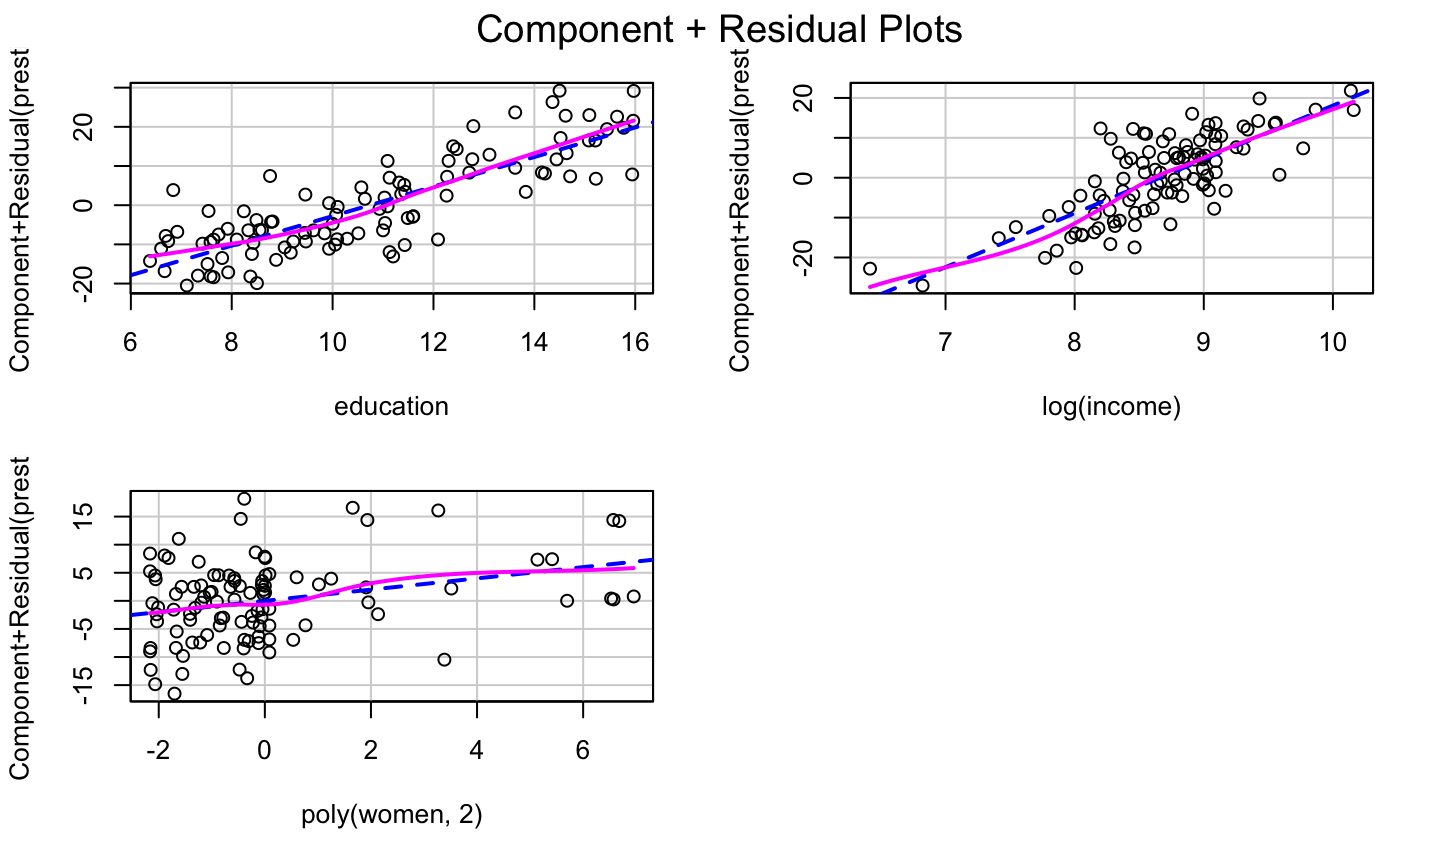
\includegraphics{error_assumption_files/figure-beamer/unnamed-chunk-17-1} \end{center}
\end{frame}

\begin{frame}[fragile]{Test for equality of variances}
\protect\hypertarget{test-for-equality-of-variances}{}
\begin{Shaded}
\begin{Highlighting}[]
\NormalTok{sample1 =}\StringTok{ }\KeywordTok{residuals}\NormalTok{(lmod)[savings}\OperatorTok{$}\NormalTok{pop15}\OperatorTok{\textgreater{}}\DecValTok{35}\NormalTok{]}
\NormalTok{sample2 =}\StringTok{ }\KeywordTok{residuals}\NormalTok{(lmod)[savings}\OperatorTok{$}\NormalTok{pop15}\OperatorTok{\textless{}}\DecValTok{35}\NormalTok{]}
\KeywordTok{var.test}\NormalTok{(sample1, sample2)}
\end{Highlighting}
\end{Shaded}

\begin{verbatim}
## 
##  F test to compare two variances
## 
## data:  sample1 and sample2
## F = 2.7851, num df = 22, denom df = 26, p-value = 0.01358
## alternative hypothesis: true ratio of variances is not equal to 1
## 95 percent confidence interval:
##  1.240967 6.430238
## sample estimates:
## ratio of variances 
##           2.785067
\end{verbatim}
\end{frame}

\begin{frame}{Checking Normality Assumption}
\protect\hypertarget{checking-normality-assumption}{}
A q-q plot (quantile-quantile plot) of the residuals can be used to
assess the assumption of normal errors.

\begin{itemize}
\item
  A q-q plot compares the residuals to ``ideal'' observations from a
  normal distribution.
\item
  The sorted residuals are plotted against
  \(\phi^{-1}\left(\frac{i}{n+1}\right)\) for \(i=1,2,\dots ,n\), where
  \(\phi^{-1}\) is the inverse cdf (quantile) function of a standard
  normal distribution.
\item
  If the residuals are distributed similarly to observations coming from
  a normal distribution, then the points of a q-q plot will lie
  approximately in a straight line at a 45 degree angle.
\end{itemize}
\end{frame}

\begin{frame}{Example (Normal)}
\protect\hypertarget{example-normal}{}
\begin{center}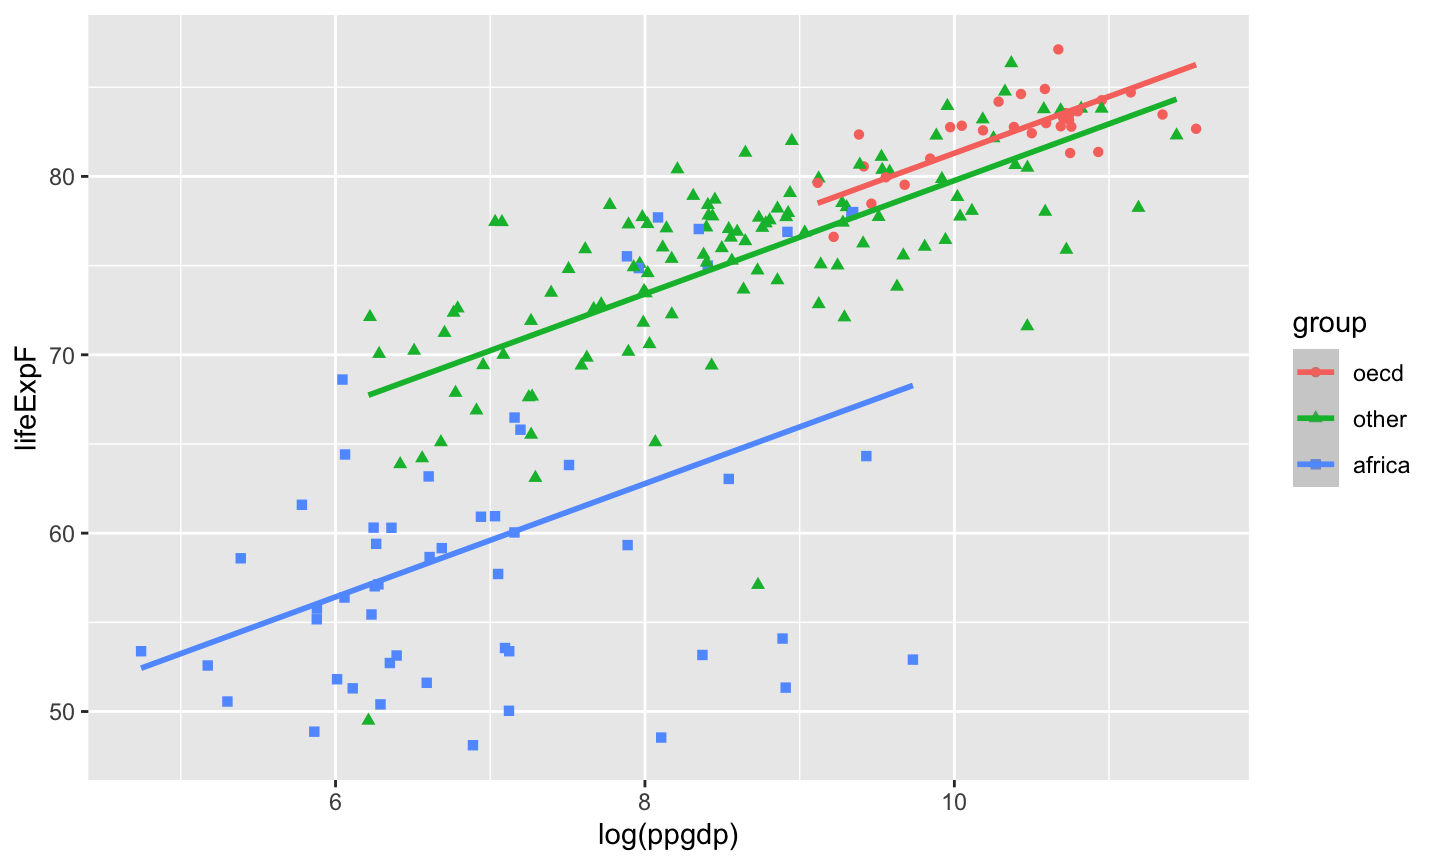
\includegraphics{error_assumption_files/figure-beamer/unnamed-chunk-19-1} \end{center}
\end{frame}

\begin{frame}{Limitation of Boxplots and histogram}
\protect\hypertarget{limitation-of-boxplots-and-histogram}{}
Histograms and boxplots are not as useful for checking normality as a
q-q plot.

\begin{itemize}
\tightlist
\item
  Boxplots can obscure a lot of information.
\item
  The shape of a histogram strongly depends on the number and size of
  the bins.
\end{itemize}
\end{frame}

\begin{frame}{Example}
\protect\hypertarget{example}{}
\begin{center}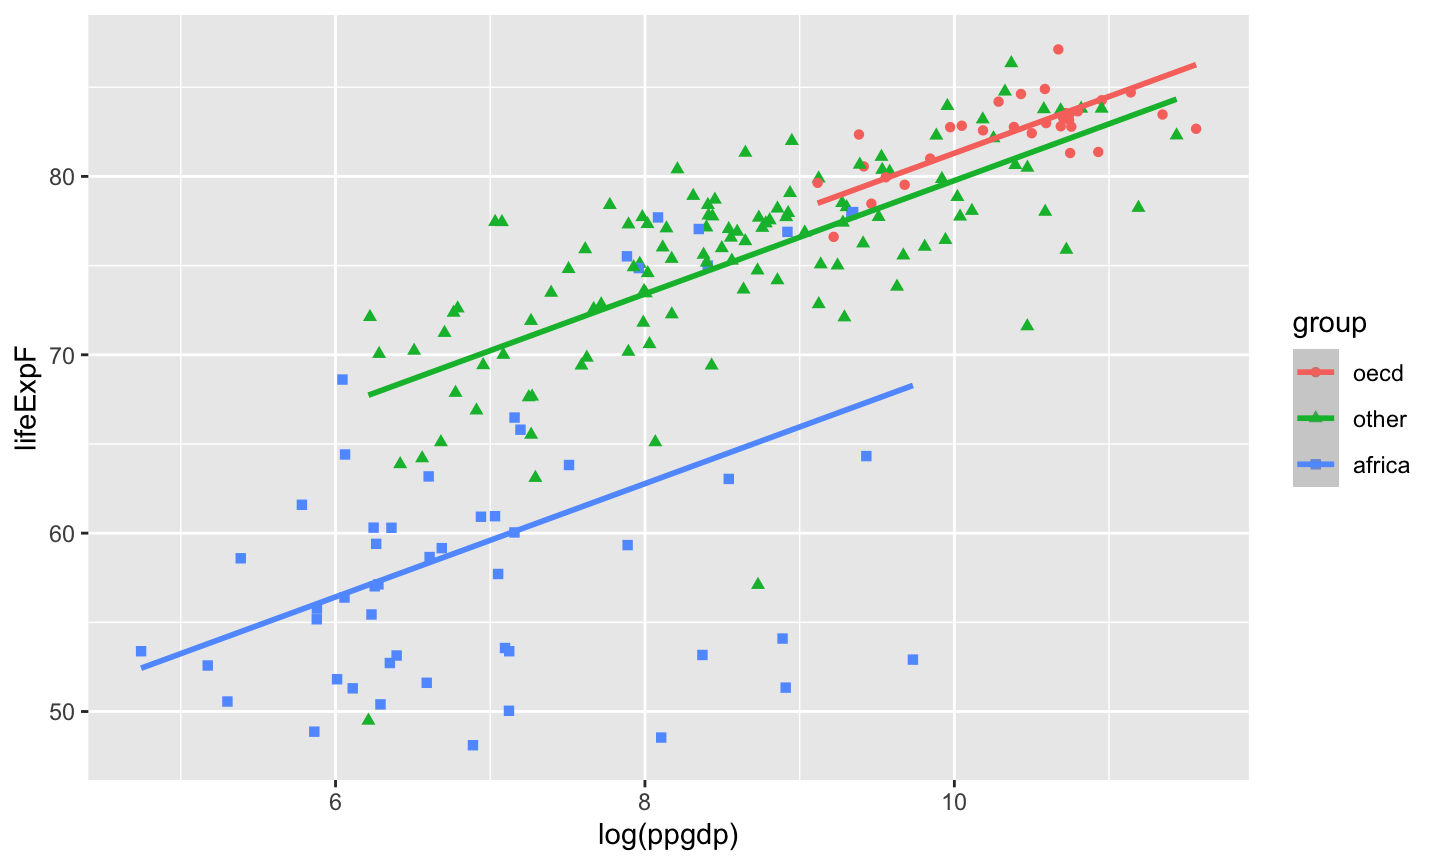
\includegraphics{error_assumption_files/figure-beamer/unnamed-chunk-20-1} \end{center}
\end{frame}

\begin{frame}{Shapiro-Wilk test}
\protect\hypertarget{shapiro-wilk-test}{}
A formal test of normality can be performed using the Shapiro-Wilk test.

\begin{itemize}
\tightlist
\item
  The null hypothesis of the Shapiro-Wilk test is that the residuals are
  a random sample from a normal distribution.\\
\item
  The alternative is that the residuals are not a sample from a normal
  distribution.
\item
  A statistical decision is made using the usual approach with p-values.
\end{itemize}

While the Shapiro-Wilk test is a tidy way to assess normality, it is not
as flexible as the q-q plot.

\begin{itemize}
\tightlist
\item
  It also does not suggest a way to correct the problem.
\item
  It is easily influenced by the number of observations so that even
  minor departures from normality are detected, even when there is
  little reason to abandon the least squares approach.
\end{itemize}
\end{frame}

\begin{frame}{When the errors are nonnormal:}
\protect\hypertarget{when-the-errors-are-nonnormal}{}
\begin{itemize}
\tightlist
\item
  Estimates will still be unbiased (assuming the model is correct and
  the error mean is zero).
\item
  Tests and confidence intervals will not be exact, but the central
  limit theorem says that the intervals and tests will be increasingly
  accurate as the sample size increases.
\item
  The consequences can generally be ignored for short-tailed
  distributions.
\item
  For skewed errors, a transformation may solve the problem.
\item
  For heavy-tailed errors, it is best to use robust methods that give
  less weight to outlying observations.
\item
  You may consider a different model. The problem may not be present in
  a different model.
\end{itemize}
\end{frame}

\begin{frame}[fragile]{Savings Example}
\protect\hypertarget{savings-example-2}{}
\begin{Shaded}
\begin{Highlighting}[]
\KeywordTok{qqPlot}\NormalTok{(lmod)}
\end{Highlighting}
\end{Shaded}

\begin{center}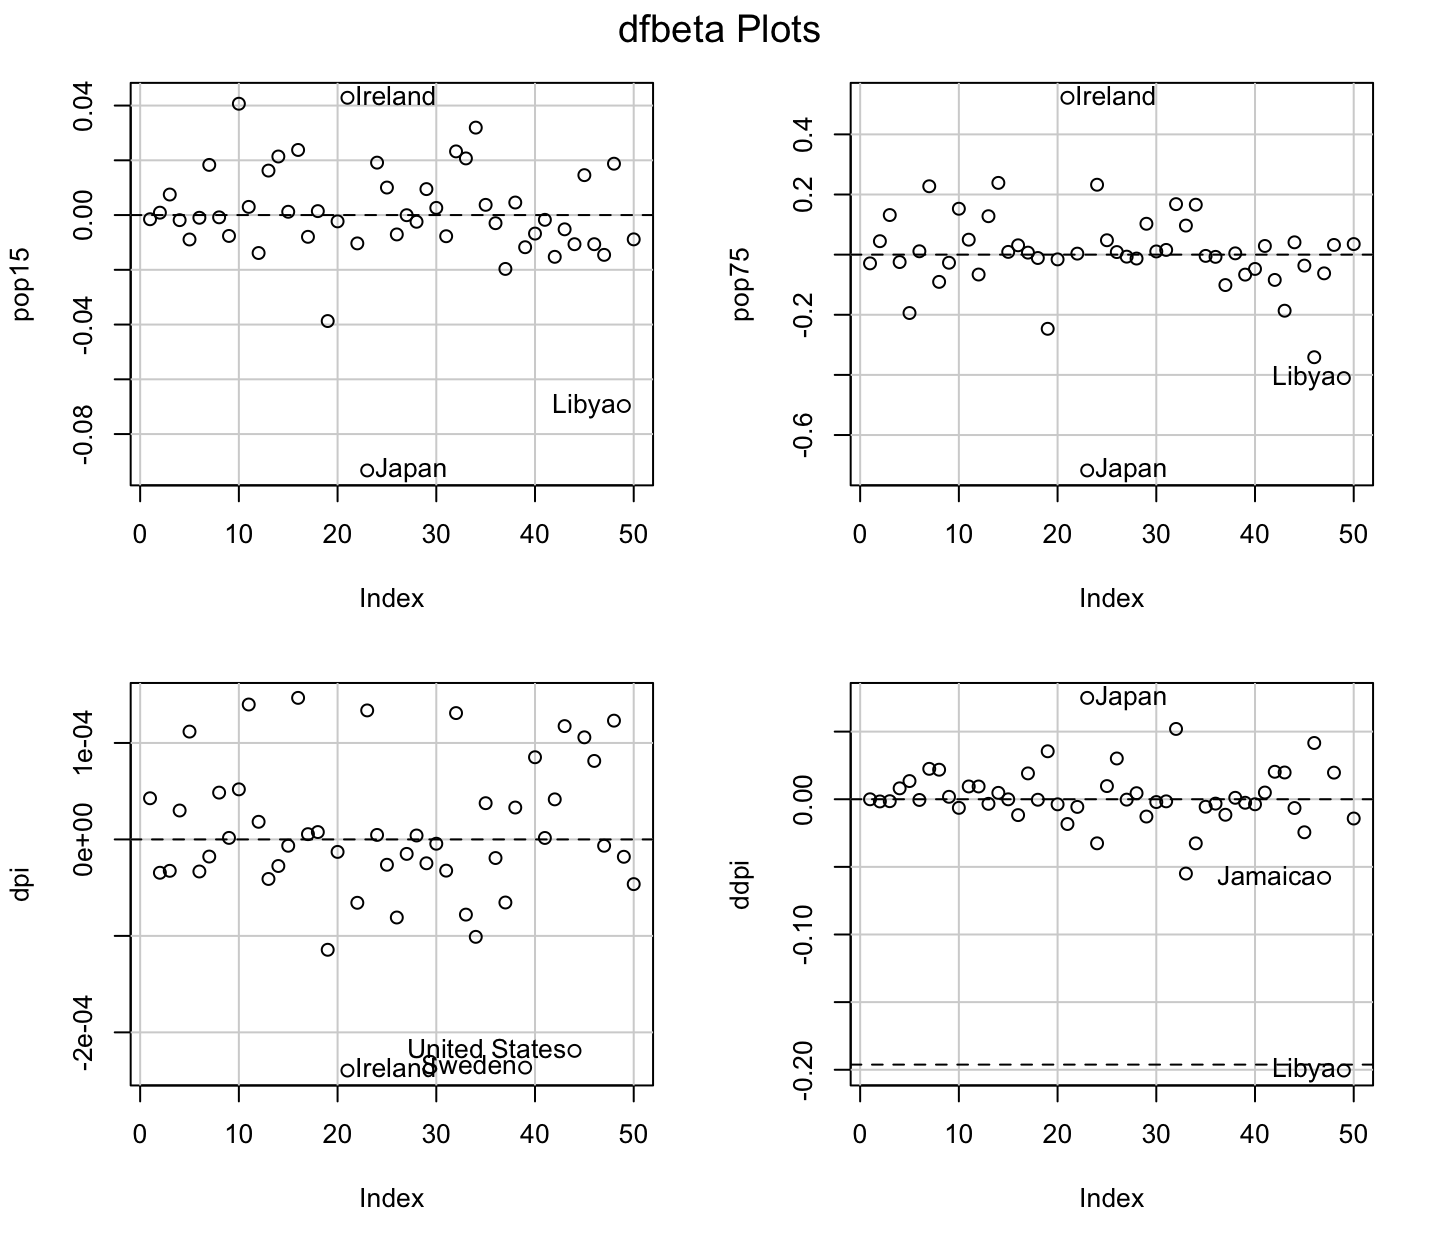
\includegraphics{error_assumption_files/figure-beamer/unnamed-chunk-21-1} \end{center}

\begin{verbatim}
##  Chile Zambia 
##      7     46
\end{verbatim}
\end{frame}

\begin{frame}[fragile]{Savings Example}
\protect\hypertarget{savings-example-3}{}
\begin{Shaded}
\begin{Highlighting}[]
\KeywordTok{shapiro.test}\NormalTok{(}\KeywordTok{residuals}\NormalTok{(lmod))}
\end{Highlighting}
\end{Shaded}

\begin{verbatim}
## 
##  Shapiro-Wilk normality test
## 
## data:  residuals(lmod)
## W = 0.98698, p-value = 0.8524
\end{verbatim}
\end{frame}

\begin{frame}{Checking for uncorrelated errors}
\protect\hypertarget{checking-for-uncorrelated-errors}{}
It is difficult to check for correlated errors because there are so many
possible patterns of correlation that may occur.

\begin{itemize}
\tightlist
\item
  The structure of temporal or spatial data make this easier to check.
\end{itemize}

If the errors are uncorrelated, then the residuals are typically close
to uncorrelated.
\end{frame}

\begin{frame}{Uncorrelated errors}
\protect\hypertarget{uncorrelated-errors}{}
A plot of \(\hat{\epsilon}\) versus time should be a random scatter of
points if the errors are uncorrelated.

\begin{itemize}
\tightlist
\item
  Correlation among the errors is suggested when these plots have a
  clear pattern, e.g., lots of positive or negative residuals strung
  together or strings of residuals with alternating signs.
\end{itemize}

A plot of \(\hat{\epsilon}_{i+1}\) versus \(\hat{\epsilon}_i\) for
\(i=1,\dots,n-1\), should be a random scatter of points if the errors
are uncorrelated.

\begin{itemize}
\tightlist
\item
  If the errors are positively correlated, we expect this plot to have a
  positive slope among the points.
\item
  If the errors are negatively correlated, we expect this plot to have a
  negative slope among the points.
\end{itemize}
\end{frame}

\begin{frame}[fragile]{Example: Global warming}
\protect\hypertarget{example-global-warming}{}
The issue of global warming has attracted significant interest in recent
years. Reliable records of annual temperatures taken with thermometers
are only available back to the 1850s. Information about temperatures
prior to this can be extracted from proxies such as tree rings. We can
build a linear model to predict temperature since 1856 and then
subsequently use this to predict earlier temperatures based on proxy
information. The data we use here are included in the \texttt{globwarm}
data set in the \texttt{faraway} package. The data are derived from
Jones and Mann (2004).
\end{frame}

\begin{frame}[fragile]{Model}
\protect\hypertarget{model}{}
Consider a model of temperature regressed on eight proxies.

\begin{itemize}
\item
  There are some missing values for \texttt{nhtemp} prior to 1856, so
  these observations are (automatically) omitted (by R) from our model.
\item
  We then plot the residuals vs time.
\end{itemize}

\begin{Shaded}
\begin{Highlighting}[]
\KeywordTok{data}\NormalTok{(globwarm,}\DataTypeTok{package=}\StringTok{"faraway"}\NormalTok{)}
\NormalTok{lmod =}\StringTok{ }\KeywordTok{lm}\NormalTok{(nhtemp }\OperatorTok{\textasciitilde{}}\StringTok{ }\NormalTok{wusa }\OperatorTok{+}\StringTok{ }\NormalTok{jasper }\OperatorTok{+}\StringTok{ }\NormalTok{westgreen }\OperatorTok{+}
\StringTok{          }\NormalTok{chesapeake }\OperatorTok{+}\StringTok{ }\NormalTok{tornetrask }\OperatorTok{+}\StringTok{ }\NormalTok{urals }\OperatorTok{+}\StringTok{ }
\StringTok{          }\NormalTok{mongolia }\OperatorTok{+}\StringTok{ }\NormalTok{tasman, }\DataTypeTok{data =}\NormalTok{ globwarm)}
\end{Highlighting}
\end{Shaded}
\end{frame}

\begin{frame}[fragile]{residuals vs time}
\protect\hypertarget{residuals-vs-time}{}
\begin{Shaded}
\begin{Highlighting}[]
\KeywordTok{plot}\NormalTok{(}\KeywordTok{residuals}\NormalTok{(lmod) }\OperatorTok{\textasciitilde{}}\StringTok{ }\NormalTok{year, }
     \DataTypeTok{data =} \KeywordTok{na.omit}\NormalTok{(globwarm), }\DataTypeTok{ylab =} \StringTok{"residuals"}\NormalTok{)}
\KeywordTok{abline}\NormalTok{(}\DataTypeTok{h =} \DecValTok{0}\NormalTok{)}
\end{Highlighting}
\end{Shaded}

\begin{center}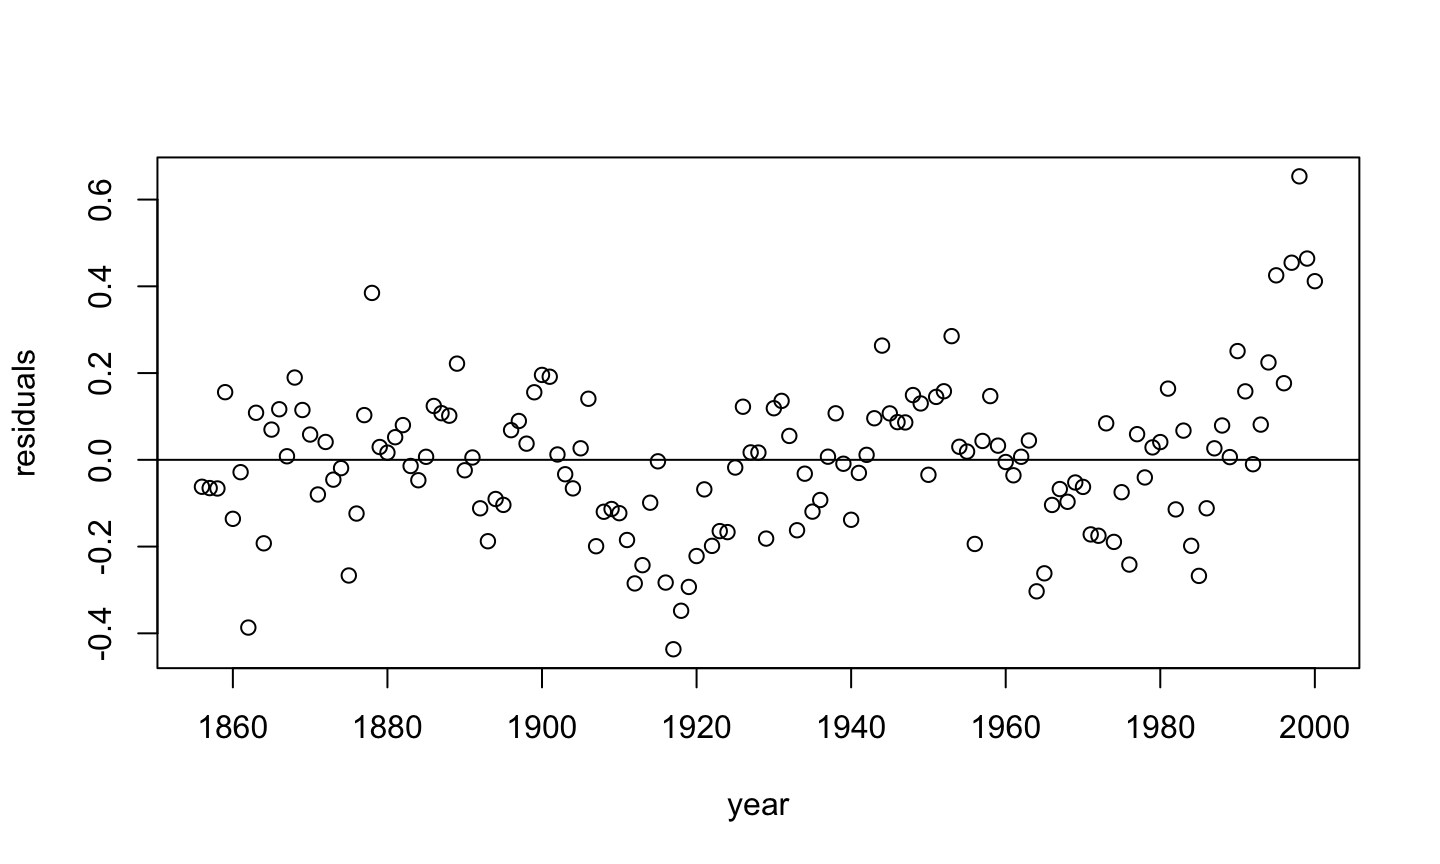
\includegraphics{error_assumption_files/figure-beamer/unnamed-chunk-24-1} \end{center}
\end{frame}

\begin{frame}{What we see}
\protect\hypertarget{what-we-see}{}
If the errors are uncorrelated, we expect a random scatter of points
around \(\hat{\epsilon}=0\), which is certainly not the case here.

The cyclical pattern suggests positive serial correlation.

\begin{itemize}
\tightlist
\item
  Another approach to check for serial correlation is to plot successive
  pairs of residuals.
\end{itemize}
\end{frame}

\begin{frame}[fragile]{Serial Correlation}
\protect\hypertarget{serial-correlation}{}
\begin{Shaded}
\begin{Highlighting}[]
\NormalTok{n =}\StringTok{ }\KeywordTok{nobs}\NormalTok{(lmod)}
\KeywordTok{plot}\NormalTok{(}\KeywordTok{tail}\NormalTok{(}\KeywordTok{residuals}\NormalTok{(lmod), n }\OperatorTok{{-}}\StringTok{ }\DecValTok{1}\NormalTok{) }\OperatorTok{\textasciitilde{}}\StringTok{ }
\StringTok{     }\KeywordTok{head}\NormalTok{(}\KeywordTok{residuals}\NormalTok{(lmod), n }\OperatorTok{{-}}\StringTok{ }\DecValTok{1}\NormalTok{), }
     \DataTypeTok{xlab =} \KeywordTok{expression}\NormalTok{(}\KeywordTok{hat}\NormalTok{(epsilon)[i]),}
     \DataTypeTok{ylab =}\KeywordTok{expression}\NormalTok{(}\KeywordTok{hat}\NormalTok{(epsilon)[i}\OperatorTok{+}\DecValTok{1}\NormalTok{]))}
\KeywordTok{abline}\NormalTok{(}\DataTypeTok{h=} \DecValTok{0}\NormalTok{ , }\DataTypeTok{v =} \DecValTok{0}\NormalTok{, }\DataTypeTok{col =} \KeywordTok{grey}\NormalTok{(}\FloatTok{0.75}\NormalTok{))}
\end{Highlighting}
\end{Shaded}

\begin{center}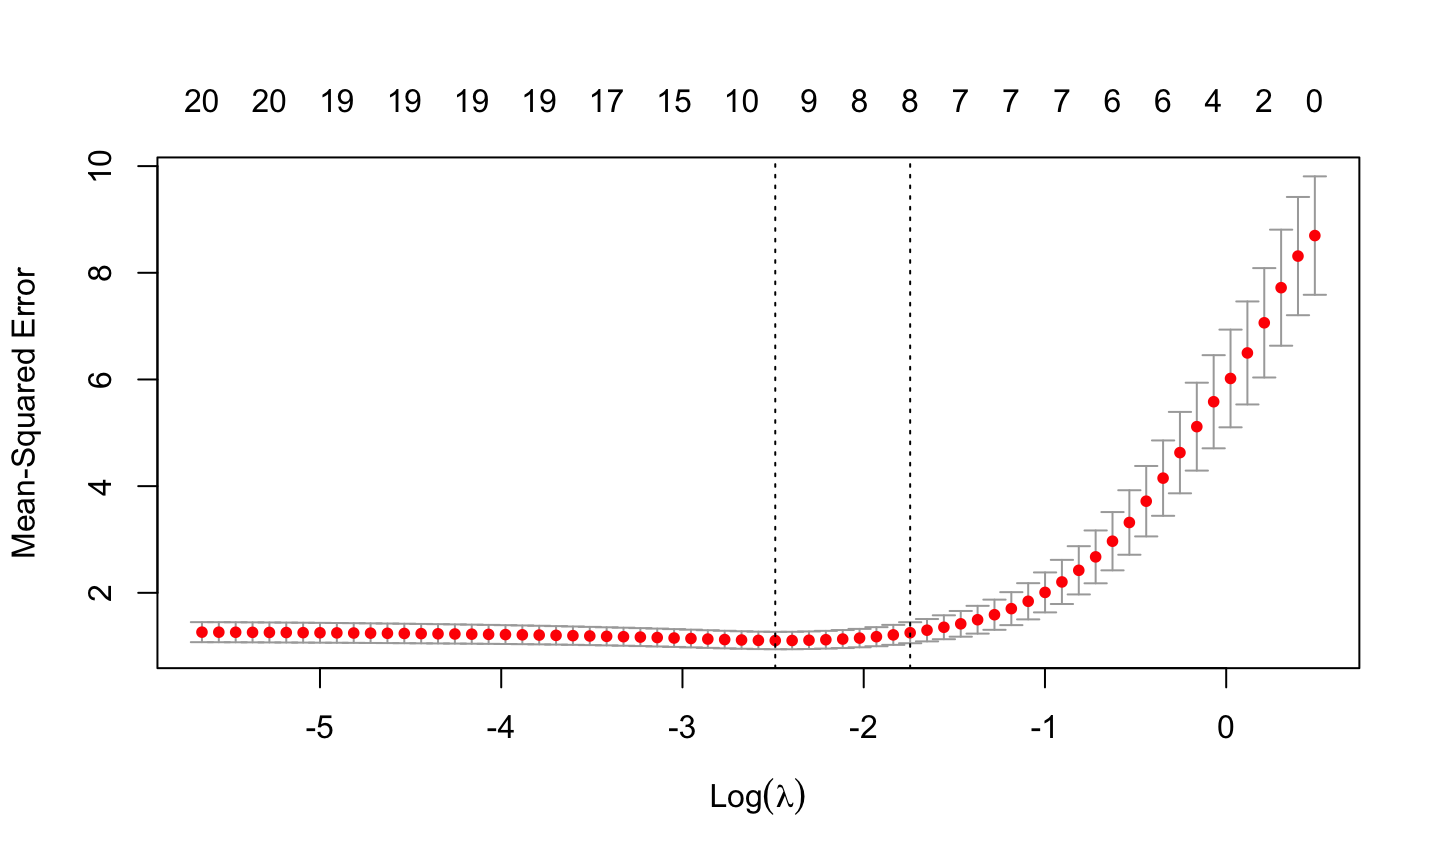
\includegraphics{error_assumption_files/figure-beamer/unnamed-chunk-25-1} \end{center}
\end{frame}

\begin{frame}{Durbin-Watson}
\protect\hypertarget{durbin-watson}{}
The positive linear trend in the previous plot suggests positive serial
correlation.

A formal test of serial correlation between residuals is the
Durbin-Watson test. The Durbin-Watson test decides between:

\[H_0:\ \rho=0 \text{ versus } H_a:\ \rho>0,\rho<0,or \rho\neq 0\]

where \(\rho\) is the temporal correlation between successive residuals.

The Durbin-Watson test uses the statistic

\[DW = \frac{\sum_{i=2}^n \left(\hat{\epsilon}_i - \hat{\epsilon}_{i-1}\right)^2}{\sum_{i=1}^n \hat{\epsilon}_i^2}\]
\end{frame}

\begin{frame}[fragile]{Durbin-Watson Test}
\protect\hypertarget{durbin-watson-test}{}
Under the null hypothesis of uncorrelated errors, the test statistic
follows a linear combination of \(\chi^2\) distributions. The test is
implemented in the lmtest package.

\begin{Shaded}
\begin{Highlighting}[]
\KeywordTok{library}\NormalTok{(lmtest)}
\KeywordTok{dwtest}\NormalTok{(nhtemp }\OperatorTok{\textasciitilde{}}\StringTok{ }\NormalTok{wusa }\OperatorTok{+}\StringTok{ }\NormalTok{jasper }\OperatorTok{+}\StringTok{ }\NormalTok{westgreen }\OperatorTok{+}\StringTok{ }\NormalTok{chesapeake }\OperatorTok{+}\StringTok{ }\NormalTok{tornetrask }\OperatorTok{+}\StringTok{ }\NormalTok{urals }\OperatorTok{+}\StringTok{ }\NormalTok{mongolia }\OperatorTok{+}\StringTok{ }\NormalTok{tasman, }\DataTypeTok{data=}\NormalTok{globwarm)}
\end{Highlighting}
\end{Shaded}

\begin{verbatim}
## 
##  Durbin-Watson test
## 
## data:  nhtemp ~ wusa + jasper + westgreen + chesapeake + tornetrask +     urals + mongolia + tasman
## DW = 0.81661, p-value = 1.402e-15
## alternative hypothesis: true autocorrelation is greater than 0
\end{verbatim}
\end{frame}

\begin{frame}{Comment on autocorrelation}
\protect\hypertarget{comment-on-autocorrelation}{}
Generalized least squares (which takes into account dependence) can be
used for data with correlated errors.

When there is no apparent temporal or spatial link between observations,
it is almost impossible to check for correlation between errors.

\begin{itemize}
\tightlist
\item
  On the other hand, there is generally no reason to suspect it either!
\end{itemize}
\end{frame}

\begin{frame}{Summary}
\protect\hypertarget{summary}{}
Summary of methods for checking error assumptions

\begin{itemize}
\tightlist
\item
  Mean-zero error assumption:

  \begin{itemize}
  \tightlist
  \item
    Plot of residuals versus fitted values
  \end{itemize}
\item
  Constant error variance assumption:

  \begin{itemize}
  \tightlist
  \item
    Plot of residuals versus fitted values
  \item
    Plot of √(\textbar ϵ ̂\textbar) versus fitted values.
  \end{itemize}
\item
  Normal error assumption:

  \begin{itemize}
  \tightlist
  \item
    q-q of residuals
  \item
    Shapiro-wilk test
  \end{itemize}
\item
  Autocorrelated errors:

  \begin{itemize}
  \tightlist
  \item
    Plot of residuals versus time
  \item
    Plot of successive pairs of residuals
  \item
    Durbin-Watson test
  \end{itemize}
\end{itemize}
\end{frame}

\begin{frame}[fragile]{Summary of R function}
\protect\hypertarget{summary-of-r-function}{}
Summary of useful R functions for checking error assumptions

Residuals:

\begin{itemize}
\tightlist
\item
  \texttt{residuals(lmod)} extracts the OLS residuals.
\item
  \texttt{rstandard(lmod)} extracts the standardized residuals.
\item
  \texttt{rstudent(lmod)} extracts the studentized residuals.
\end{itemize}

Mean-zero error assumption:

\begin{itemize}
\tightlist
\item
  \texttt{car::residualPlot} constructs a plot of the residuals versus
  fitted values.
\item
  \texttt{plot(lmod,\ which\ =\ 1)} constructs a plot of the residuals
  versus fitted values.
\end{itemize}
\end{frame}

\begin{frame}[fragile]{Summary of R function}
\protect\hypertarget{summary-of-r-function-1}{}
Constant error variance assumption:

\begin{itemize}
\tightlist
\item
  \texttt{car::residualPlots} constructs a plots of the residuals versus
  each predictor and the residuals versus the fitted values.
\item
  \texttt{plot(lmod,\ which\ =\ 3)} constructs a plot of
  \(\sqrt{|\hat{\epsilon}|}\) versus the fitted values.
\end{itemize}

Normal error assumption:

\begin{itemize}
\tightlist
\item
  \texttt{car::qqPlot} constructs a q-q of the studentized residuals
  with 95\% pointwise confidence bands.
\item
  \texttt{plot(lmod,\ which\ =\ 2)} constructs a q-q plot of the
  standardized residuals.
\item
  \texttt{shapiro.test(residuals(lmod))} performs a Shapiro-Wilk test on
  the residuals.
\end{itemize}

Autocorrelated errors:

\begin{itemize}
\tightlist
\item
  \texttt{lmtest::dwtest} performs a Durbin-Watson test on the residuals
  of a fitted model.
\end{itemize}
\end{frame}

\begin{frame}{Importance of Linear Regression Assumptions}
\protect\hypertarget{importance-of-linear-regression-assumptions}{}
Some assumptions are more important than others because their violation
can cause seriously inaccurate conclusions.

We can order these assumptions according to their importance:

\begin{enumerate}
\tightlist
\item
  The systematic form of the model. If you get this seriously wrong,
  then predictions will be inaccurate and any explanation of the
  relationship between the variables may be biased in misleading ways.
\end{enumerate}
\end{frame}

\begin{frame}{Importance of Linear Regression Assumptions}
\protect\hypertarget{importance-of-linear-regression-assumptions-1}{}
\begin{enumerate}
\setcounter{enumi}{1}
\tightlist
\item
  Dependence of errors. The presence of strong dependence means that
  there is less information in the data than the sample size may
  suggest. Furthermore, there is a risk that the analyst will mistakenly
  introduce systematic components to the model in an attempt to deal
  with an unsuspected dependence in the errors. Unfortunately, it is
  difficult to detect dependence in the errors using regression
  diagnostics except in special situations such as temporal data. For
  other types of data, the analyst will need to rely on less testable
  assumptions about independence based on contextual knowledge.
\end{enumerate}
\end{frame}

\begin{frame}{Importance of Linear Regression Assumptions}
\protect\hypertarget{importance-of-linear-regression-assumptions-2}{}
\begin{enumerate}
\setcounter{enumi}{2}
\item
  Nonconstant variance. A failure to address this violation of the
  linear model assumptions may result in inaccurate inferences. In
  particular, prediction uncertainty may not be properly quantified.
  Even so, excepting serious violations, the adequacy of the inference
  may not be seriously compromised.
\item
  Normality. This is the least important assumption. For large datasets,
  the inference will be quite robust to a lack of normality as the
  central limit theorem will mean that the approximations will tend to
  be adequate. Unless the sample size is quite small or the errors very
  strongly abnormal, this assumption is not crucial to success.
\end{enumerate}
\end{frame}

\begin{frame}{Conclusion}
\protect\hypertarget{conclusion}{}
Although it is not part of regression diagnostics, it is worth
mentioning that an even more important assumption is that the data at
hand are relevant to the question of interest.

This requires some qualitative judgment and is not checkable by plots or
tests.
\end{frame}
